%%%%%%%%%%%%%%%%%%%%%%%%%%%%%%%%%%%%%%%%%%%%%%%%%%%%%%%%%%%%%%%%%%%%%%%%%%%%
% AGUJournalTemplate.tex: this template file is for articles formatted with LaTeX

%% To submit your paper:
\documentclass[draft, grl]{agujournal2019}
%\documentclass[draft,jgrga]{agutexSI2019}
\usepackage{url} %this package should fix any errors with URLs in refs.
\usepackage{lineno}
\usepackage{minted}
\usepackage{makecell}
\usepackage{natbib}
\usepackage[colorlinks=true, urlcolor=blue, linkcolor=red]{hyperref}
\usepackage{subfiles}
\usepackage{float}
\usepackage{caption}

\DeclareCaptionFormat{cancaption}{#1#2#3\par} % Normal format actually
\DeclareCaptionLabelFormat{cancaptionlabel}{#1 S#2}

%
\usepackage[inline]{trackchanges} %for better track changes. finalnew option will compile document with changes incorporated.
\usepackage{soul}

\linenumbers

%\draftfalse

\begin{document}

\journalname{Geophysical Research Letters}

\title{Supplementary Material for ``Land Processes Can Substantially Impact the Mean Climate State''
}

\authors{Claire M. Zarakas\affil{1} , 
Daniel Kennedy\affil{3}, 
Katherine Dagon\affil{3}, 
David M. Lawrence\affil{3}, 
Amy Liu\affil{1}, 
Gordon Bonan\affil{3}, 
Charles Koven\affil{4},
Danica Lombardozzi\affil{3},
and Abigail L. S. Swann\affil{1,2}}

\affiliation{1}{University of Washington, Department of Atmospheric Sciences}
\affiliation{2}{University of Washington, Department of Biology}
\affiliation{3}{National Center for Atmospheric Research}
\affiliation{4}{Lawrence Berkeley National Laboratory}

%% Corresponding Author:
%\correspondingauthor{Claire M. Zarakas}{czarakas@uw.edu}

%\begin{article}
\noindent\textbf{Contents of this file}
%%%Remove or add items as needed%%%
\begin{enumerate}
\item Text S1 to S4
\item Figures S1 to S15
\item Tables S1 to S4
%if Tables are larger than 1 page, upload as separate excel file
\end{enumerate}
\clearpage{}

\renewcommand{\thesection}{Text S\arabic{section}}

\section{Model configuration and experimental design}
\label{Text:model_configuration}
CESM PPE simulations were run using the \href{https://github.com/ESCOMP/CTSM/releases/tag/branch_tags\%2FPPE.n11_ctsm5.1.dev030}{\mintinline{Fortran}{branch_tags/PPE.n11_ctsm5.1.dev030}} tag for the Community Land Model version 5 \citep[CLM5;][]{lawrence_community_2019} and the \href{https://github.com/ESCOMP/CESM/releases/tag/cesm2.2.0}{\mintinline{Fortran}{cesm2.2.0}} tag for all other model components. The land was initialized with the spun-up land state from the default model parameterization which includes the carbon content of soil and vegetation pools. The coupled simulations use the Community Atmosphere Model 6 \citep[CAM6;][]{bogenschutz_path_2018}, and a slab ocean \citep{danabasoglu_equilibrium_2009} which is based on q-fluxes from preindustrial simulations of the full dynamic ocean model. We did not apply flux corrections, and note that the top of atmosphere energy imbalance is relatively small and changes minimally across the PPE (average=-0.157 W/m$^2$, $\sigma$=0.010 W/m$^2$; Figure S\ref{fig:supp_TOA_energy_balance}).

Each parameter perturbation simulation, which we refer to as an ensemble member, was run for 140 years under constant preindustrial greenhouse gas concentrations and land use conditions. The first 40 years were discarded as spin up, which is long enough for fast atmospheric processes, leaf area, soil moisture and temperature, and the surface ocean to largely equilibrate (Figure S\ref{fig:supp_spinup}).

\section{Parameter selection procedure}
\label{Text:parameter_selection}
We used two parameter selection criteria: (1) that parameters would likely have a large impact on the atmosphere, based on results from the CLM5 PPE, and (2) that parameters sampled different functional areas of the model. For our first criterion, we ranked all parameters based on multiple metrics of land-to-atmosphere fluxes (Table S\ref{table:metrics_of_impact}, Table S\ref{table:LH_example_rankings}), globally and for individual biomes, focusing on the quantities that the land model passes to the atmosphere model in CESM2 (Table S\ref{table:land2atm_fluxes}). We quantified parameters impact on individual biomes by classifying the land surface into the nine Whittaker biomes \citep{whittaker_communities_1975} and ice sheets based on each grid cell's mean precipitation and temperature. Out of 205 total parameters, we identified 40 parameters that appeared in the top five for more than five rankings. For our second criterion, we then grouped those top 40 parameters into functional categories, and we selected 18 parameters such that we did not sample more than four parameters from any given functional category. 

\section{Calculating the pattern of warming due to a doubling of CO$_2$}
\label{Text:doubling_CO2}
We calculated the pattern of warming due to a doubling of CO$_2$ from  two concentration-driven CESM2 simulations: one forced with preindustrial CO$_2$ concentrations of 284.7 ppm (1xCO$_2$) and one forced with a doubling of preindustrial CO$_2$, 569.4 ppm (2xCO$_2$). We ran simulations with an active land and atmosphere, and a slab ocean. We ran simulations for 120 years, and discarded the first 60 years as spin up. These CESM simulations were run using the \href{https://github.com/ESCOMP/CESM/releases/tag/cesm2_3_beta03}{\mintinline{Fortran}{cesm_2_3_beta03}} tag and \href{https://github.com/ESCOMP/CTSM/releases/tag/branch_tags%2FPPE.n08_ctsm5.1.dev030}{\mintinline{Fortran}{branch_tags/PPE.n08_ctsm5.1.dev030}} tag for CTSM. Doubling CO$_2$ drove a 5.2°C global mean temperature increase (6.5°C global mean land temperature increase), consistent with CESM2's documented high equilibrium climate sensitivity (Gettelman et al. 2019). 
\\[16pt]

\section{Disentangling drivers of land temperature and precipitation changes}
%Calculating emergent changes in land surface properties
\label{Text:land_surface properties}

We used multiple linear regression to disentangle the extent to which land precipitation ($P$) and temperature ($T_s$) changes across our coupled PPE are driven by three land surface properties: albedo ($\alpha$), evaporative fraction (EF), and a measure of aerodynamic coupling ($r_a$). First, we diagnosed $\alpha$, EF, and $r_a$ for each ensemble member of land-only PPE at each grid cell using monthly model output. We calculated $r_a$ by inverting the equation for sensible heat flux. We then use these derived changes in land-only $\alpha$, EF, $r_a$ as predictors in a multiple linear regression to predict coupled $T_s$ and P change at each point for each month. We used predictors from the land-only rather than the coupled PPE in order to remove the feedback between climate and land surface properties. In the coupled PPE, changes in land surface properties are due to both land parameter uncertainty and land responses to climate changes (e.g., precipitation changes can influence evaporative fraction), but changes in land surface properties in the land-only PPE isolate the influence of land parameter uncertainty on land surface fluxes. Because this grid cell level analysis does not account for remote or global-scale impacts of parameter perturbations, we also report results from regressions conducted using global averages. We do not perform regressions on global average land precipitation changes because the sign of precipitation changes are more regionally variable. 

We calculated the emergent changes in $r_s$ and $r_a$ by inverting the equations for sensible heat flux and latent heat flux (L).  S=($\rho C_p (T_s-T_a))/r_a$  and L=($\rho \lambda(q^* (T_s)-q_a))/(r_a+r_s )$, where $\rho$ is the air density at the lowest atmospheric level, $T_a$ is the air temperature at the lowest atmospheric level, $q_a$ is the specific humidity at the lowest atmospheric level, $T_s$ is land surface skin temperature, and $q^* (T_s)$is the saturated specific humidity at $T_s$. $C_p$ and $\lambda$ are constants, the specific heat capacity of dry air and the latent heat of vaporization, respectively. We verified our derived changes in $\alpha$, $r_s$, and $r_a$ by demonstrating that they yielded accurate reconstructions of temperature changes in the offline land-only PPE using the two-resistance method (TRM; Rigden and Li 2017). However, the TRM is ill-suited for attributing quantifying how much the changes in $\alpha$, $r_s$, and $r_a$ drive coupled temperature changes to changes in $\alpha$, $r_s$, and $r_a$ because it combines all temperature changes from atmospheric feedbacks into one term (due to change in the near-surface  air temperature $T_a$), and cannot distinguish the extent to which $T_a$ changes are driven by changes in $\alpha$, $r_s$, and $r_a$.
%\end{article}
\pagebreak
% Add discussion of robustness testing here.

%TC:ignore
\bibliography{PPE_refs}
%TC:endignore

%% ------------------------------------------------------------------------ 
%\section*{Supplemental Figures}

\captionsetup[figure]{format=cancaption,labelformat=cancaptionlabel}
\begin{figure}[htb!]
\noindent\includegraphics[width=\textwidth]{writing/figs/Figure_S1.pdf}
\caption{Maps of annual mean land temperature changes for each ensemble member, compared to the reference case with default parameterizations. Hatching indicates regions where the temperature change was insignificant at the 0.05 significance level. The percentage of land with statistically significant temperature changes is shown in parentheses, and * indicates field significance. For each grid cell, we performed a two-tailed Student’s t-test to test whether the ensemble member mean (standard deviation calculated from the distribution from interannual variability in the ensemble member mean) was different from the default mean (standard deviation calculated from the distribution from interannual variability in the default mean). We test for field significance using Walker’s test.}
\label{fig:supp_coupled_Ts_land_maps}
\end{figure}

\begin{figure}[htb!]
\noindent\includegraphics[width=\textwidth]{writing/figs/Figure_S2.pdf}
\caption{Maps of annual mean temperature changes for each ensemble member, including both land and ocean. Hatching and significance testing is as in Figure S1, but the title indicates the total percentage of the Earth surface (including land and ocean) with statistically significant temperature changes.}
\label{fig:supp_coupled_Ts_land_and_ocean_maps}
\end{figure}


\begin{figure}[htb!]
\noindent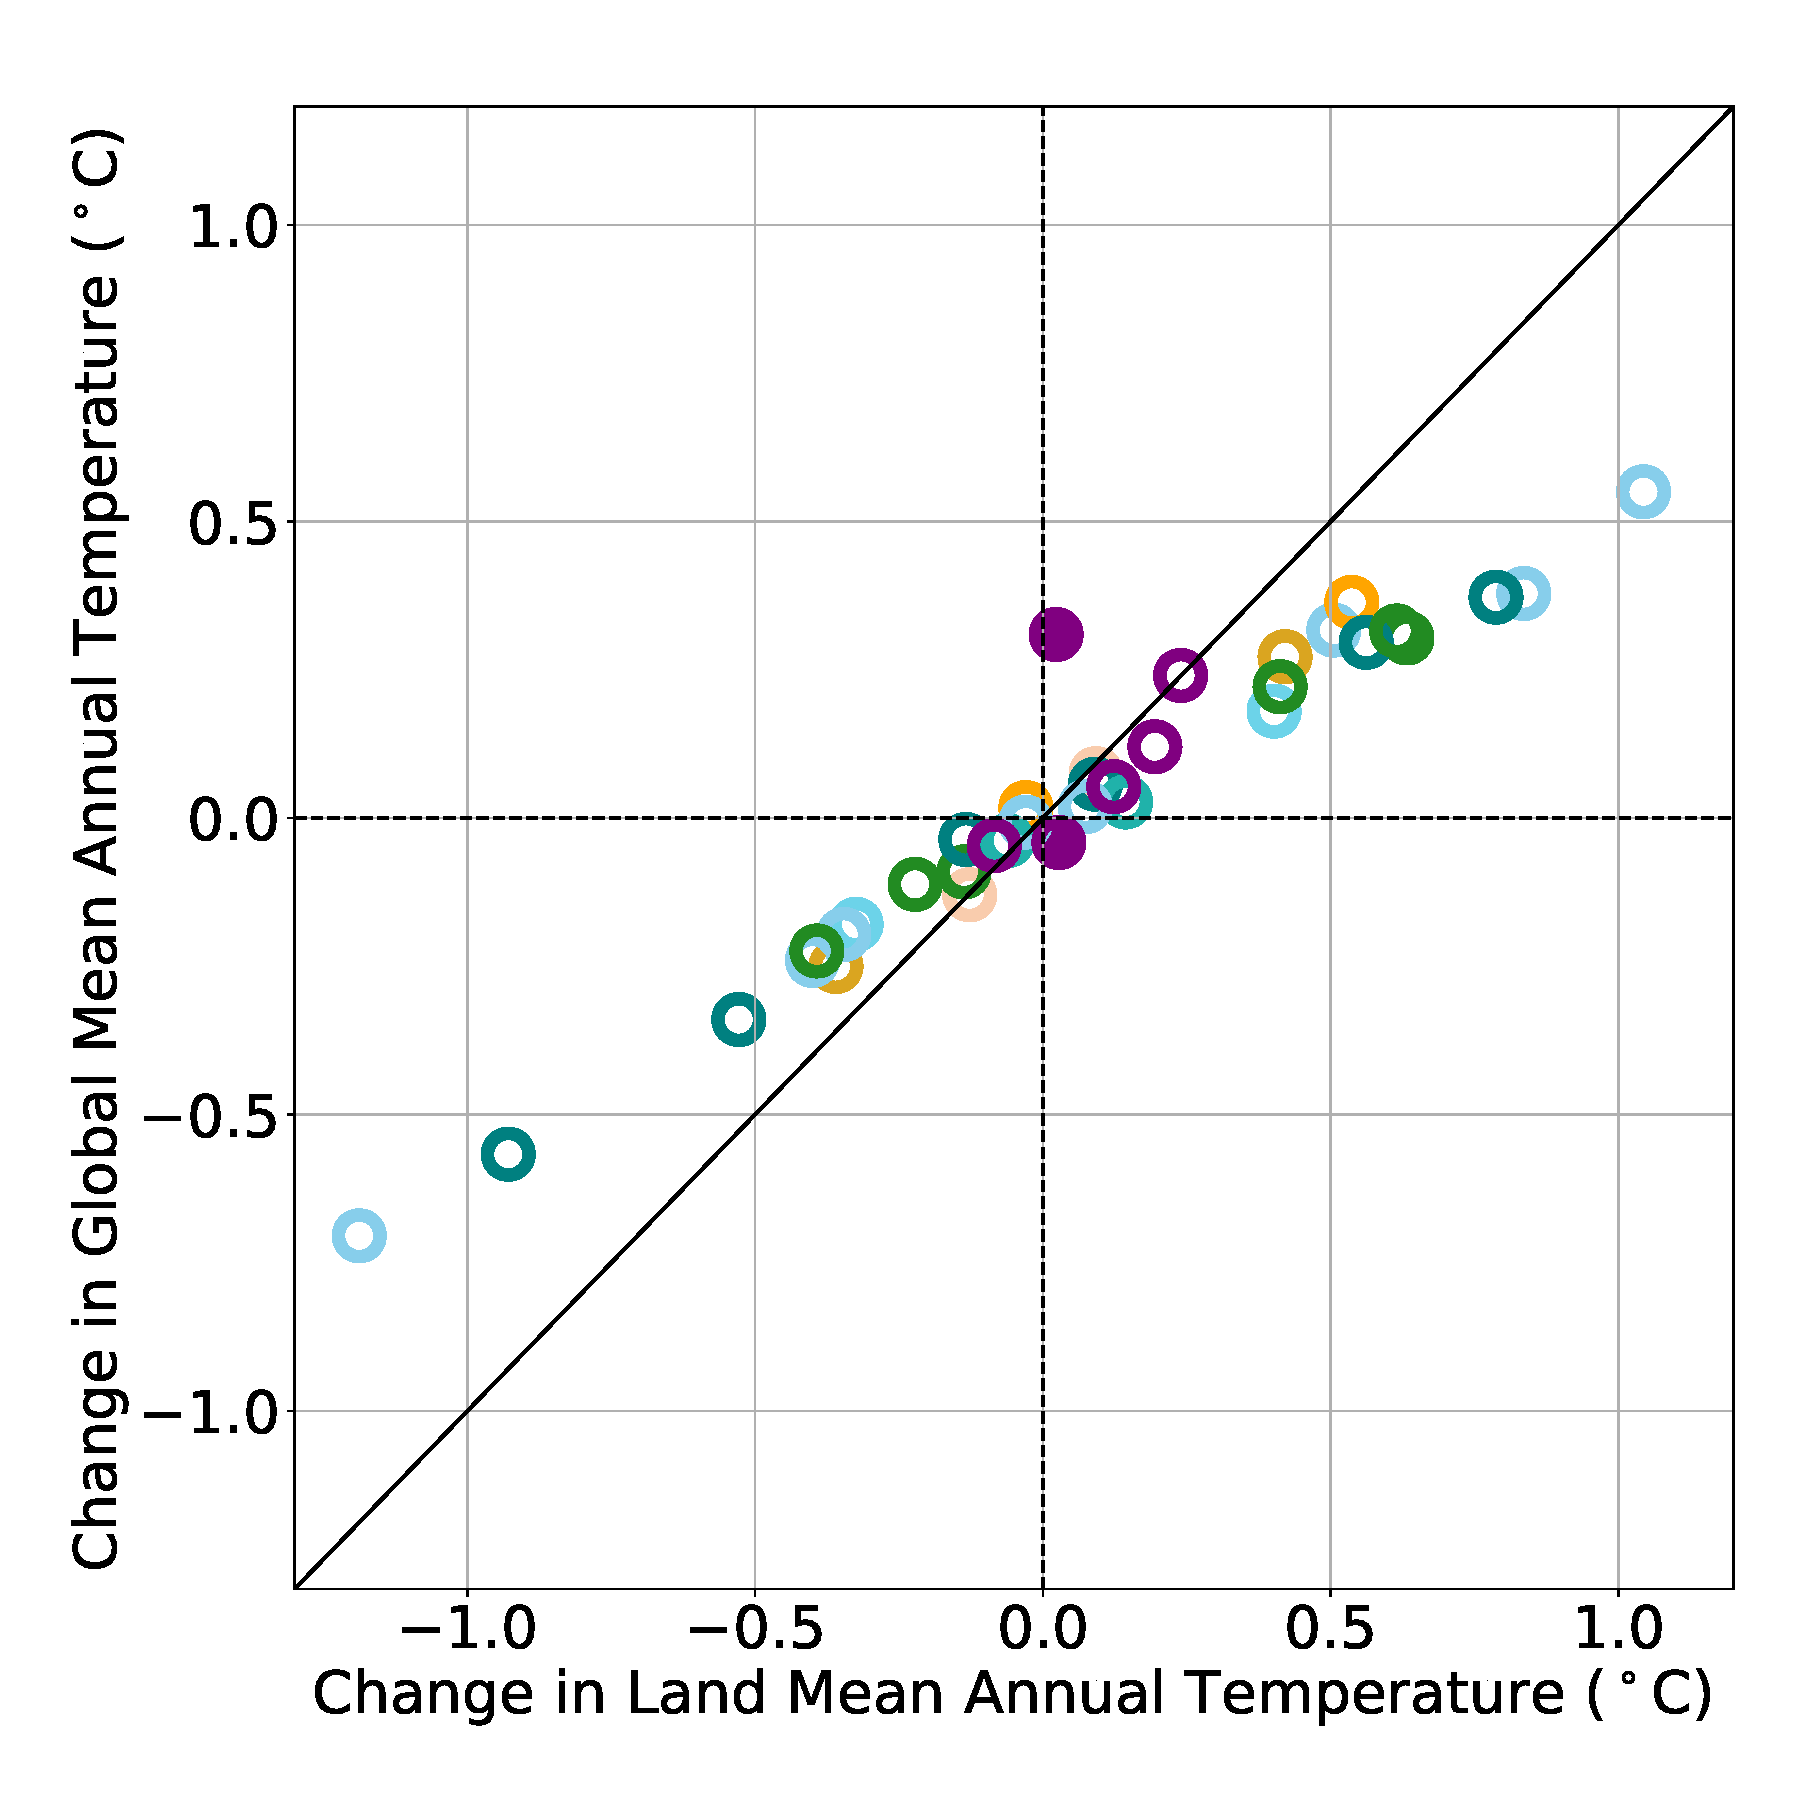
\includegraphics[width=\textwidth]{writing/figs/Figure_S3.pdf}
\caption{Correlation between the change in annual mean land temperature and annual mean global temperature (including both land and ocean). Colors indicate parameter category as in Figures 1 and 3. Because the parameter \mintinline{Fortran}{zetamaxstable} is an outlier in our PPE, it is denoted as the filled purple point.}
\label{fig:supp_coupled_Ts_land_vs_ocean_maps}
\end{figure}

\begin{figure}[htb!]
\noindent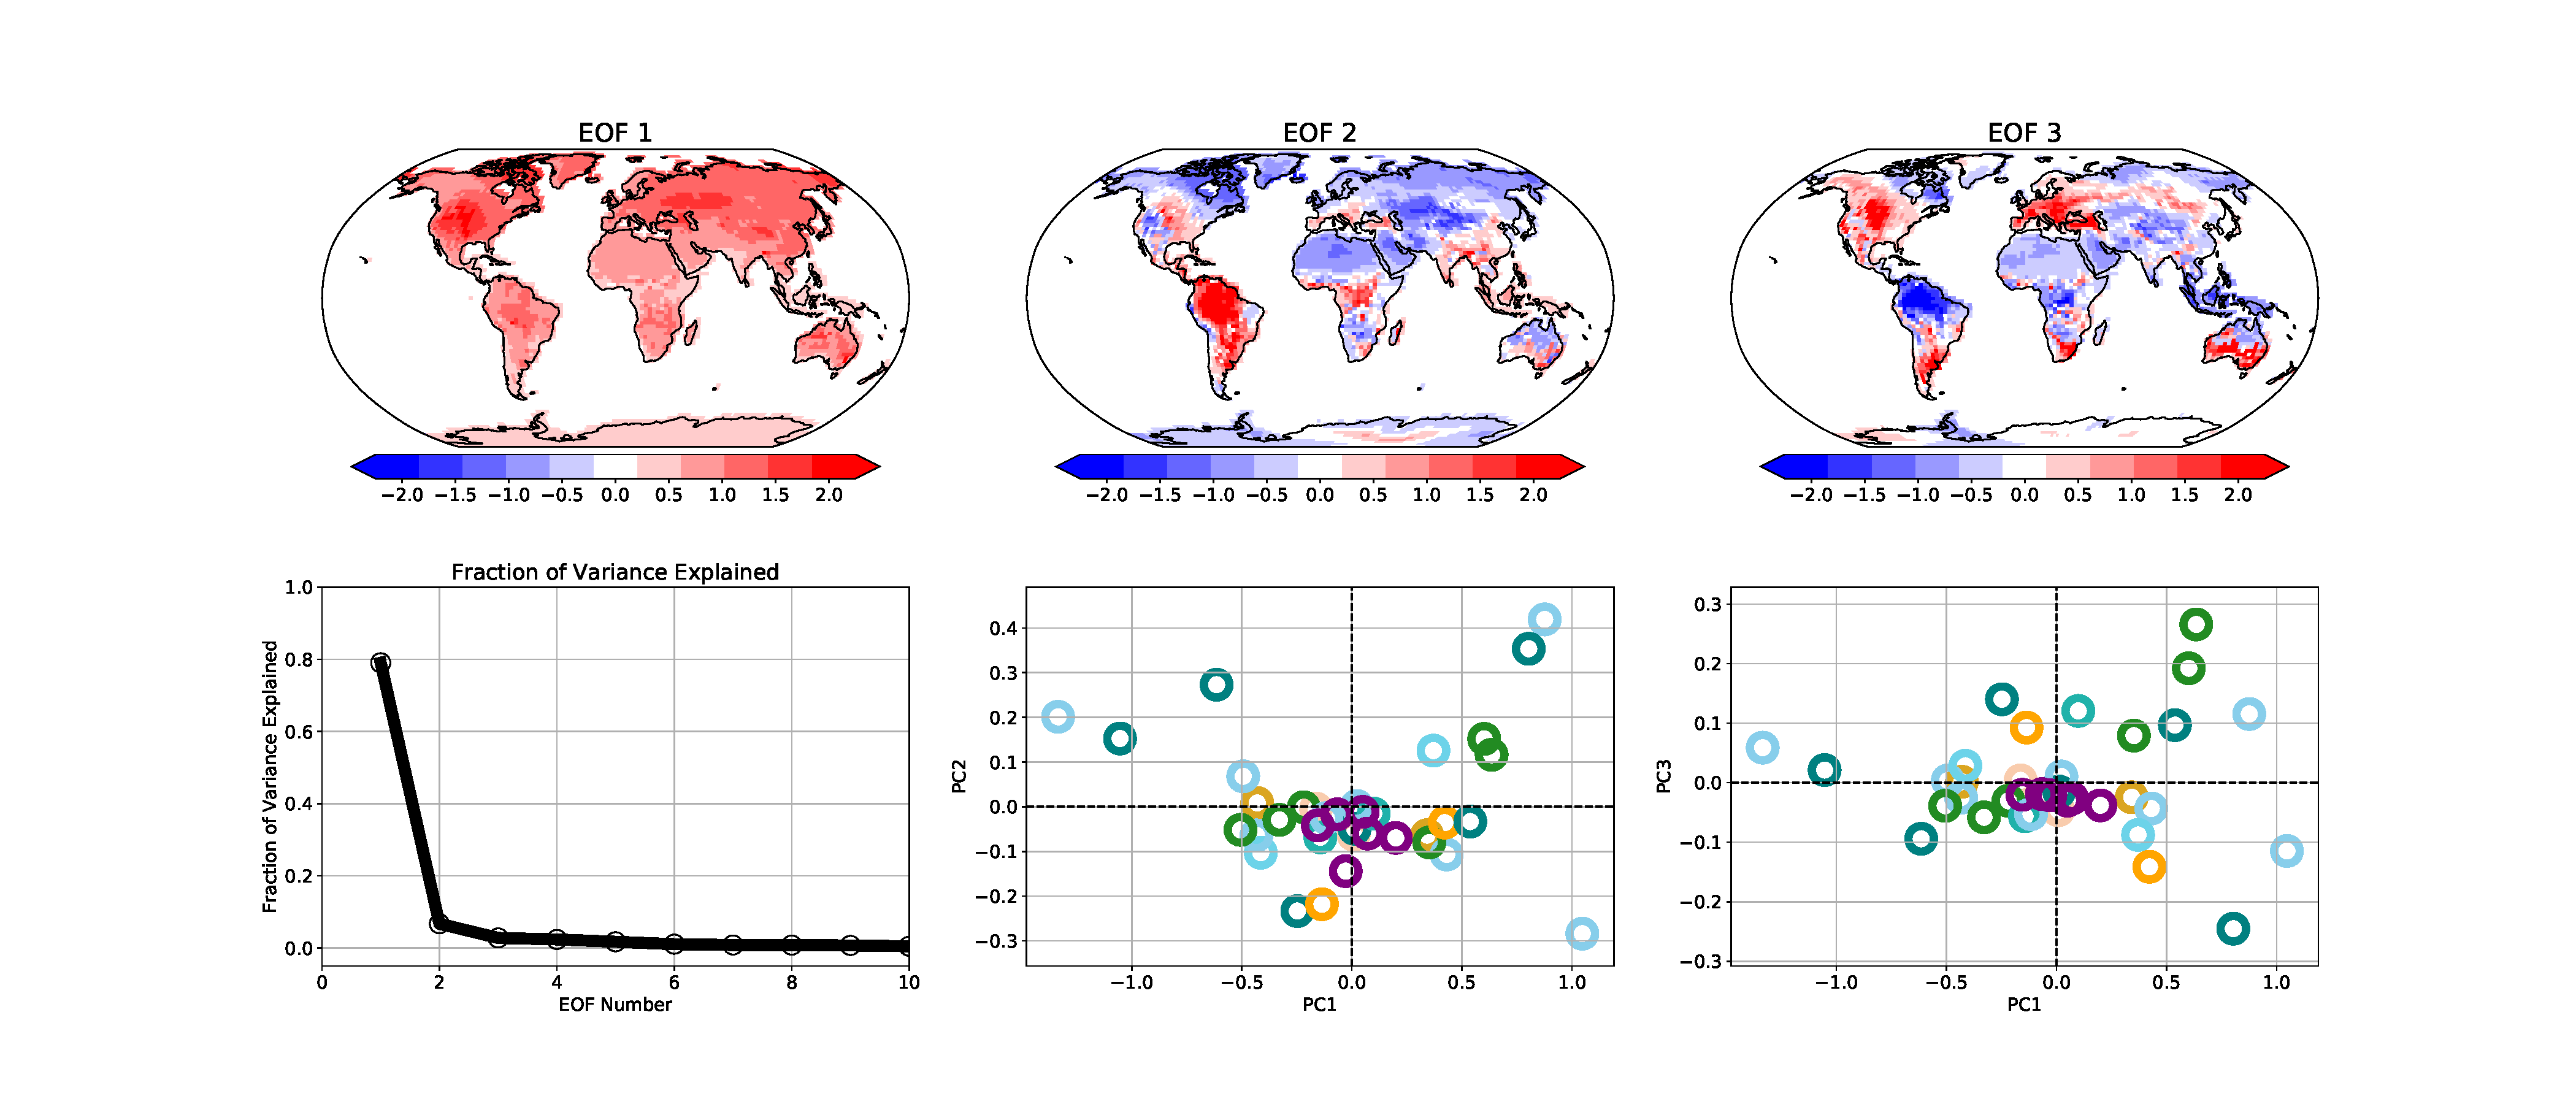
\includegraphics[width=\textwidth]{writing/figs/Figure_S_TSKIN_EOF_summary.pdf}
\caption{EOF analysis of changes in land surface temperature across the PPE. }
\label{fig:supp_EOF_analysis_Temp}
\end{figure}

\begin{figure}[htb!]
\noindent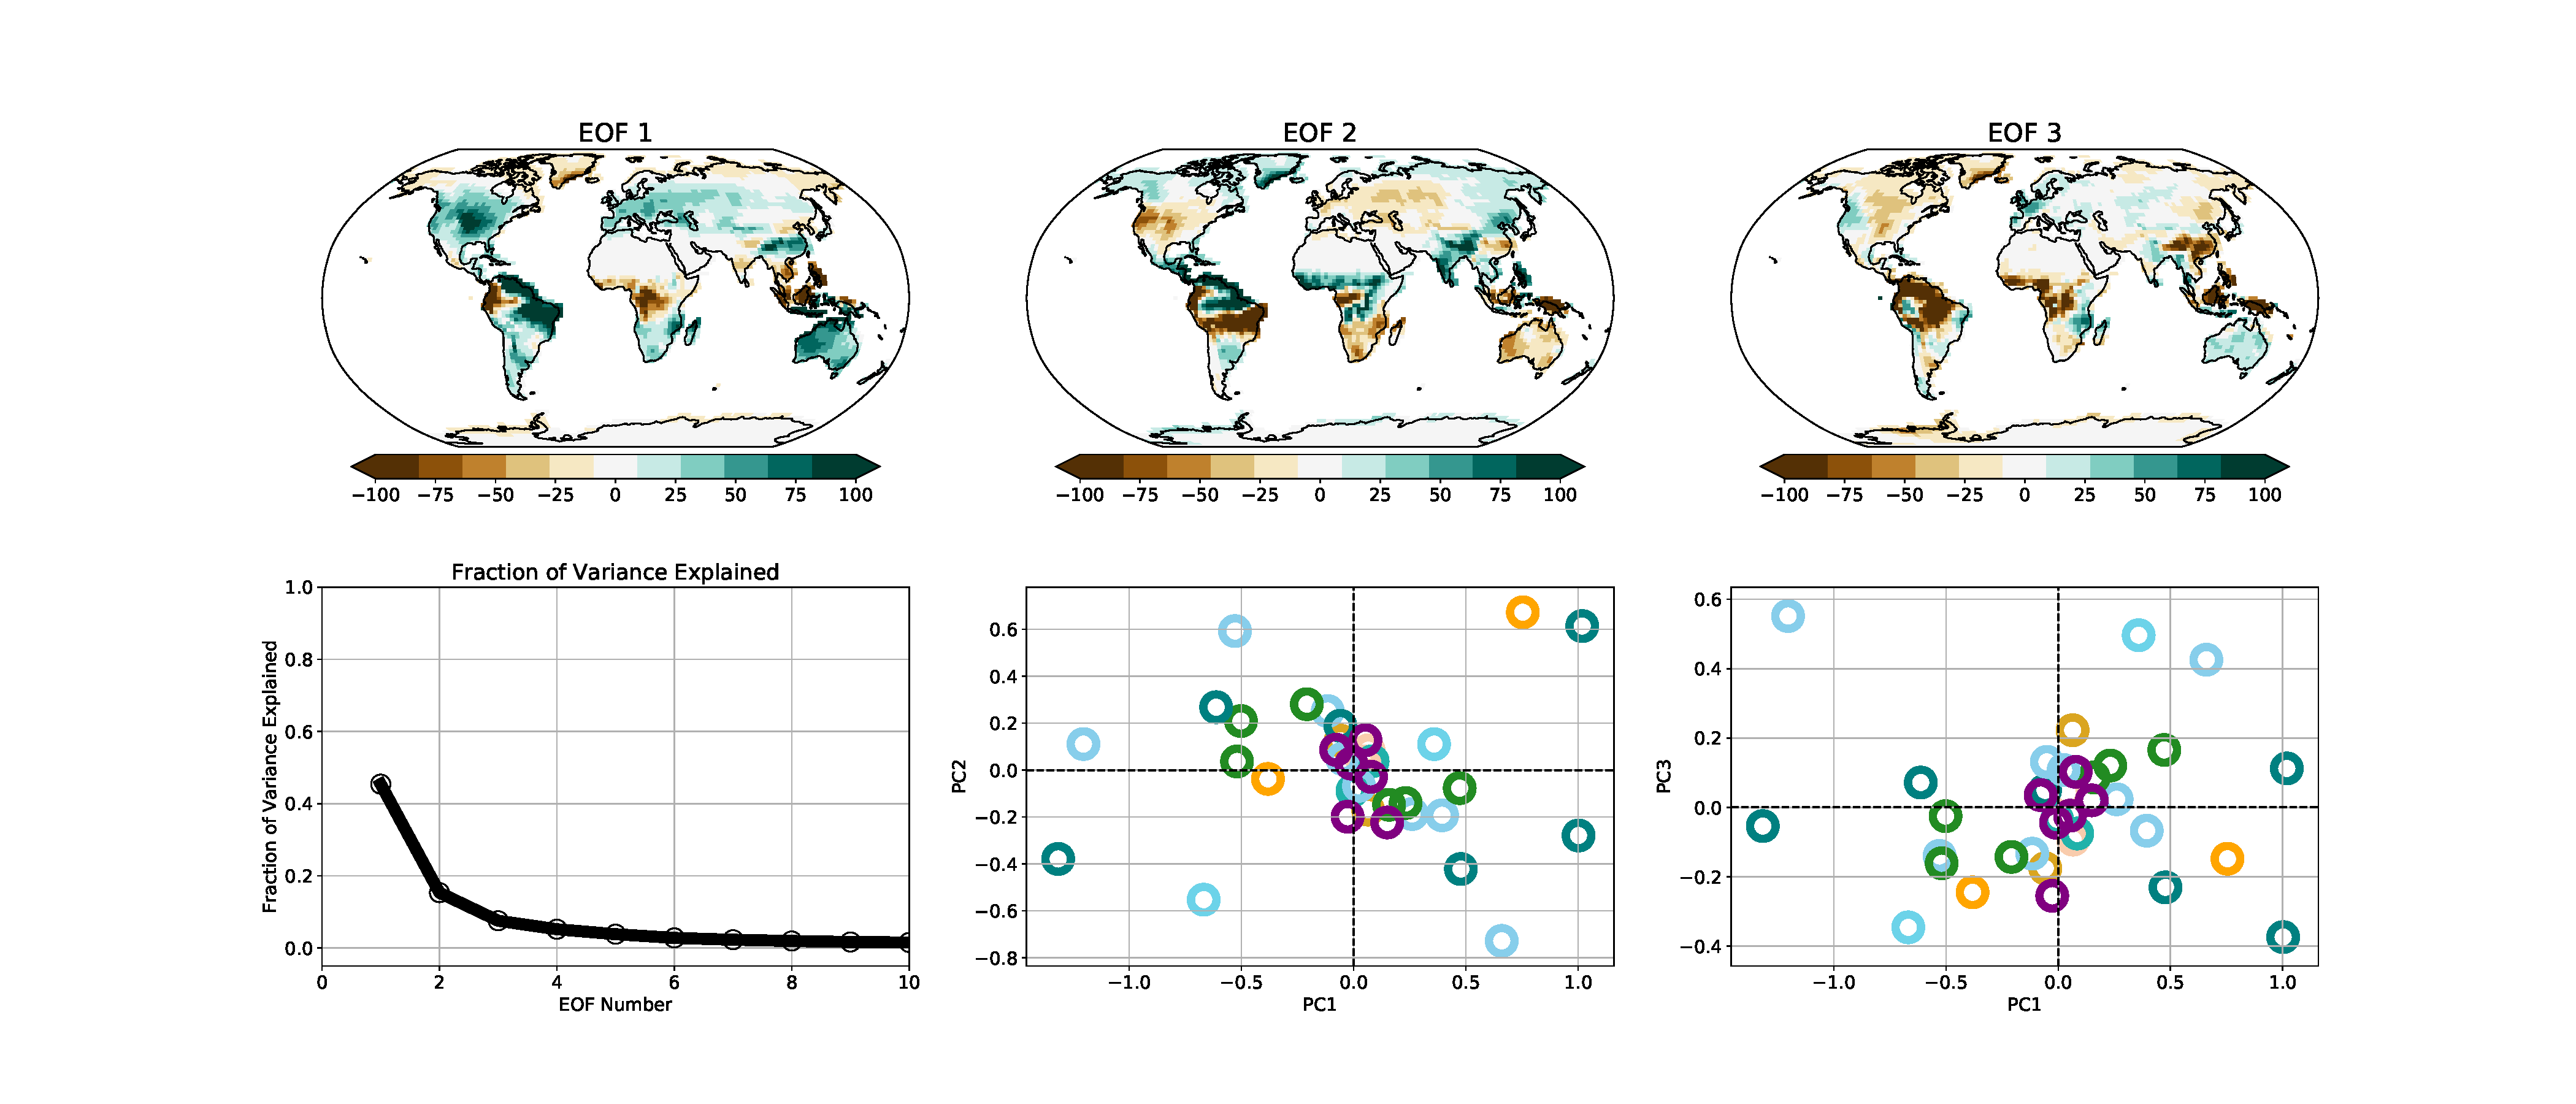
\includegraphics[width=\textwidth]{writing/figs/Figure_S_PRECT_EOF_summary.pdf}
\caption{EOF analysis of changes in land precipitation across the PPE.}
\label{fig:supp_EOF_analysis_Precip}
\end{figure}

\begin{figure}[htb!]
\noindent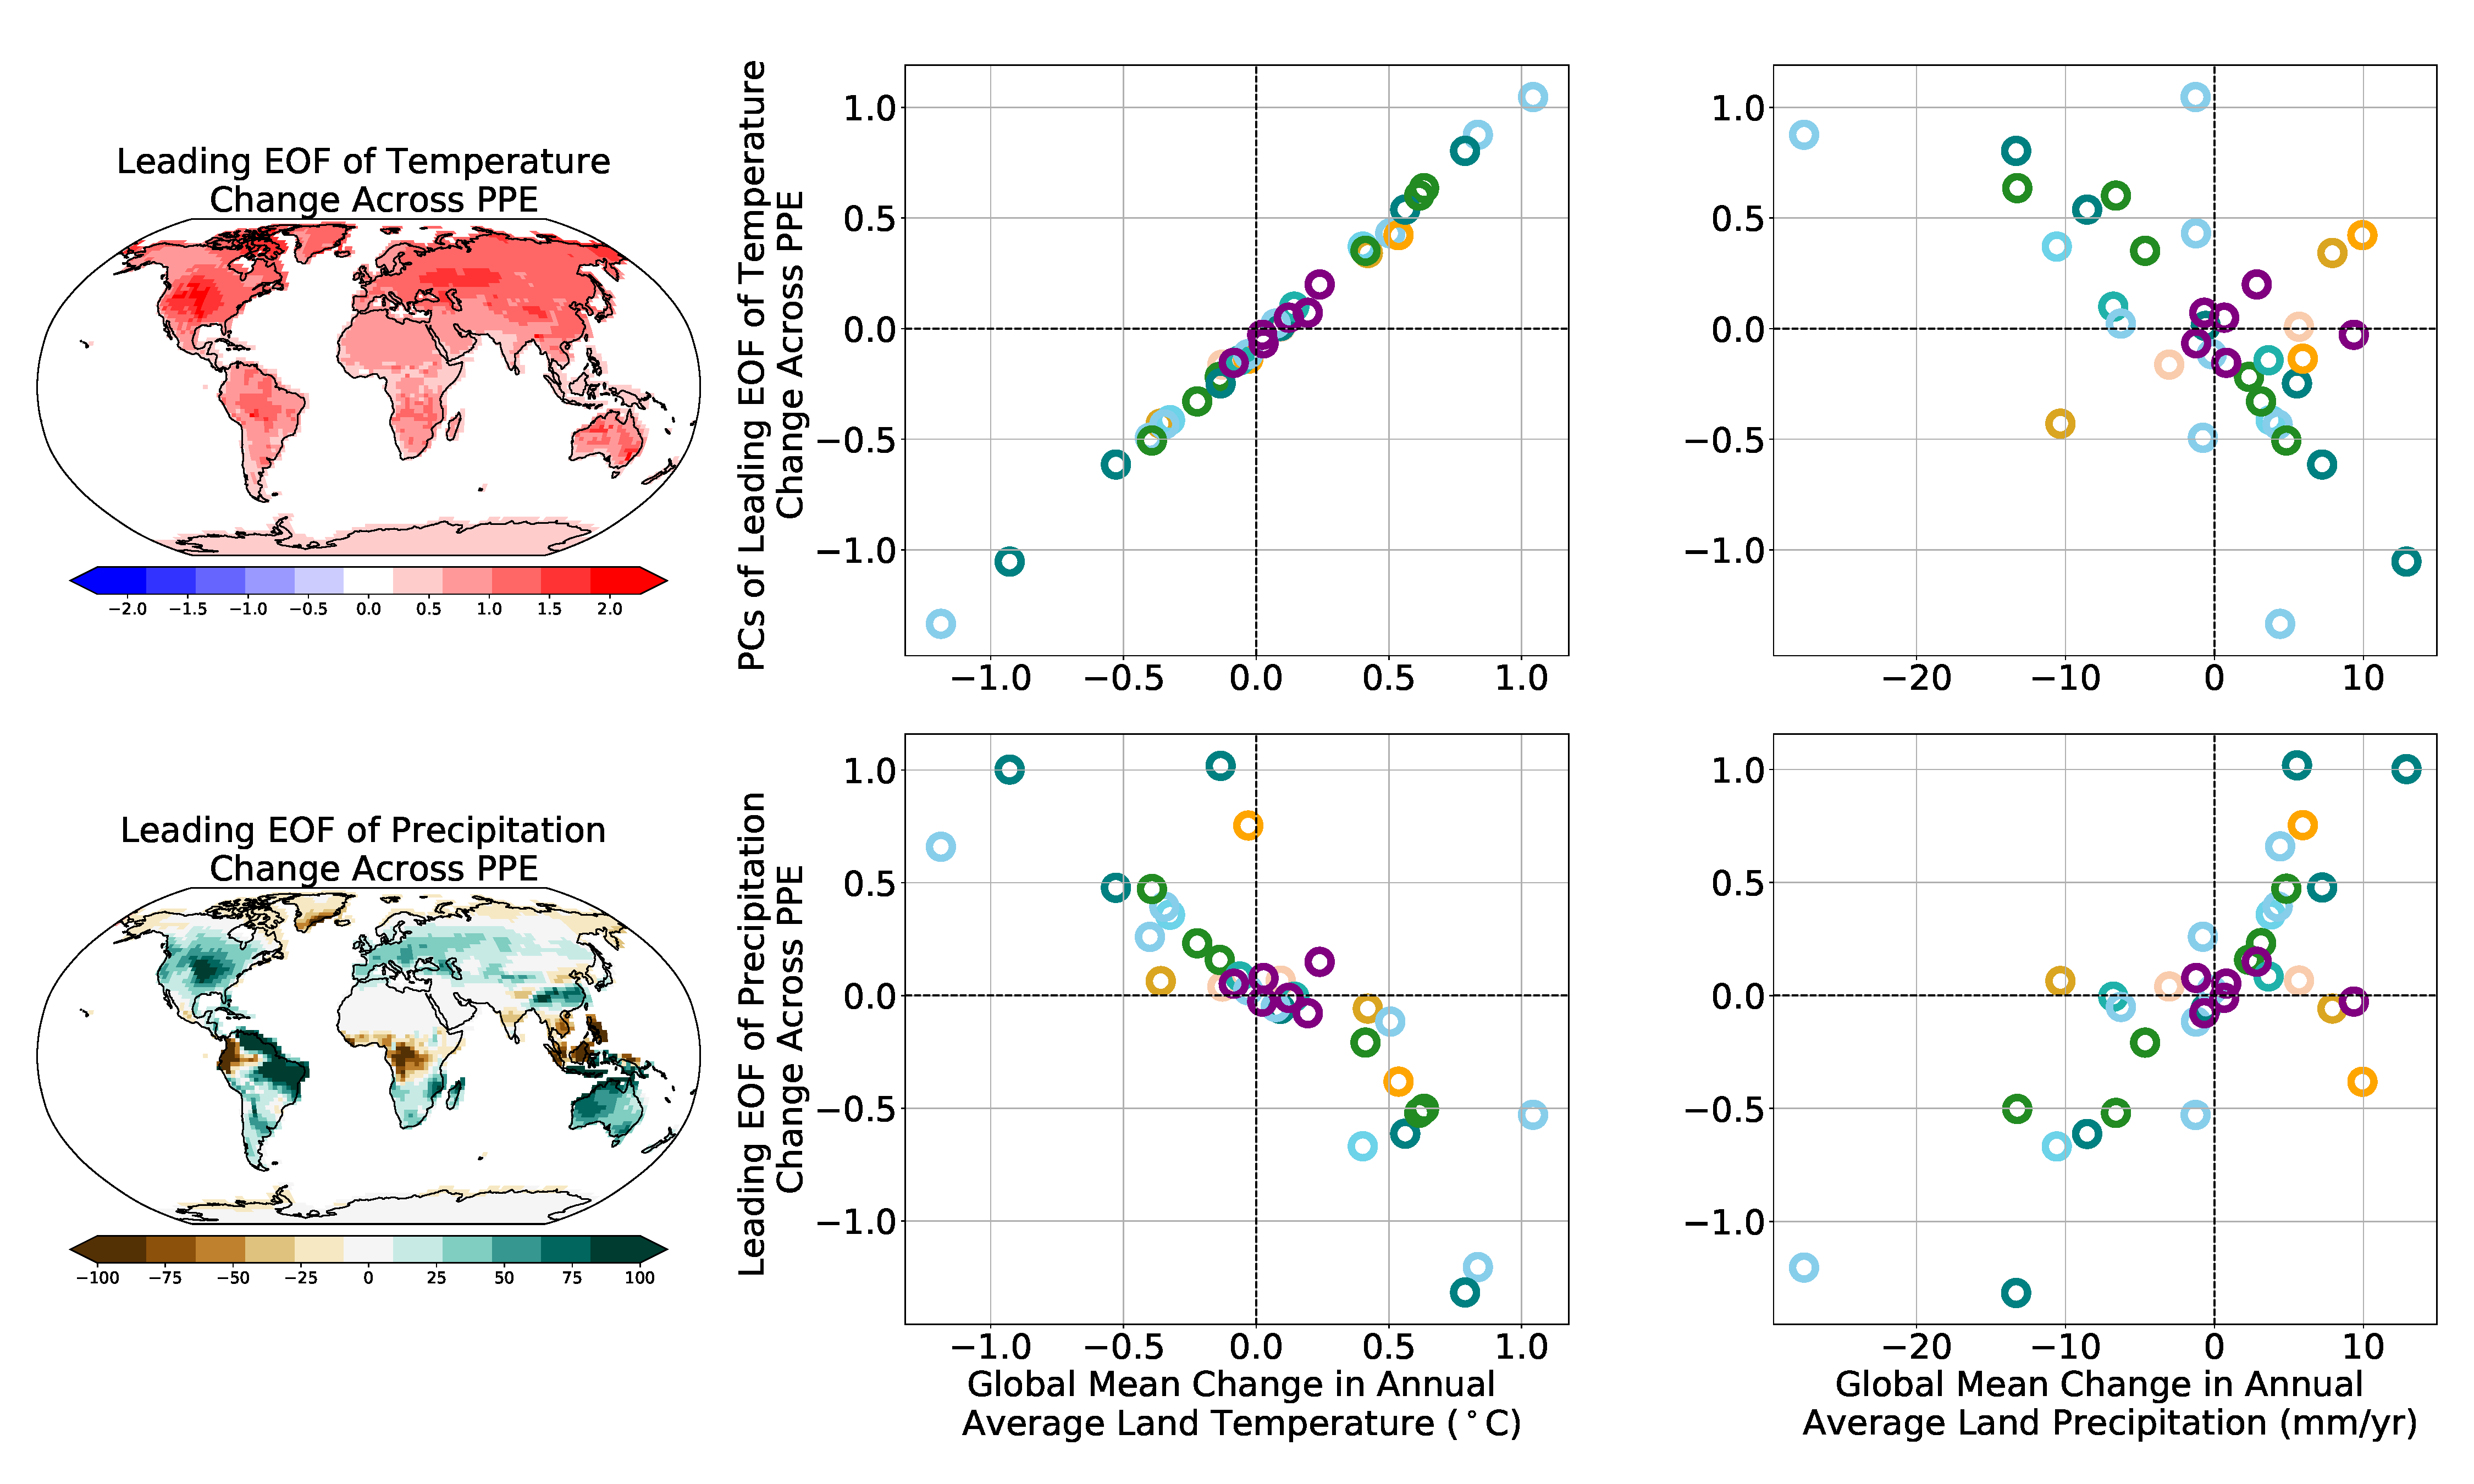
\includegraphics[width=\textwidth]{writing/figs/Figure_S_Correlation_between_EOFs_and_global_mean_changes.pdf}
\caption{Correlation between leading EOFs of annual average land and temperature changes and global mean annual average land temperature and precipitation changes across the PPE. Ensemble members are colored by parameter category, as in Figure 1.}
\label{fig:supp_EOF_globalmetric_correlation}
\end{figure}

\begin{figure}[htb!]
\centering
\noindent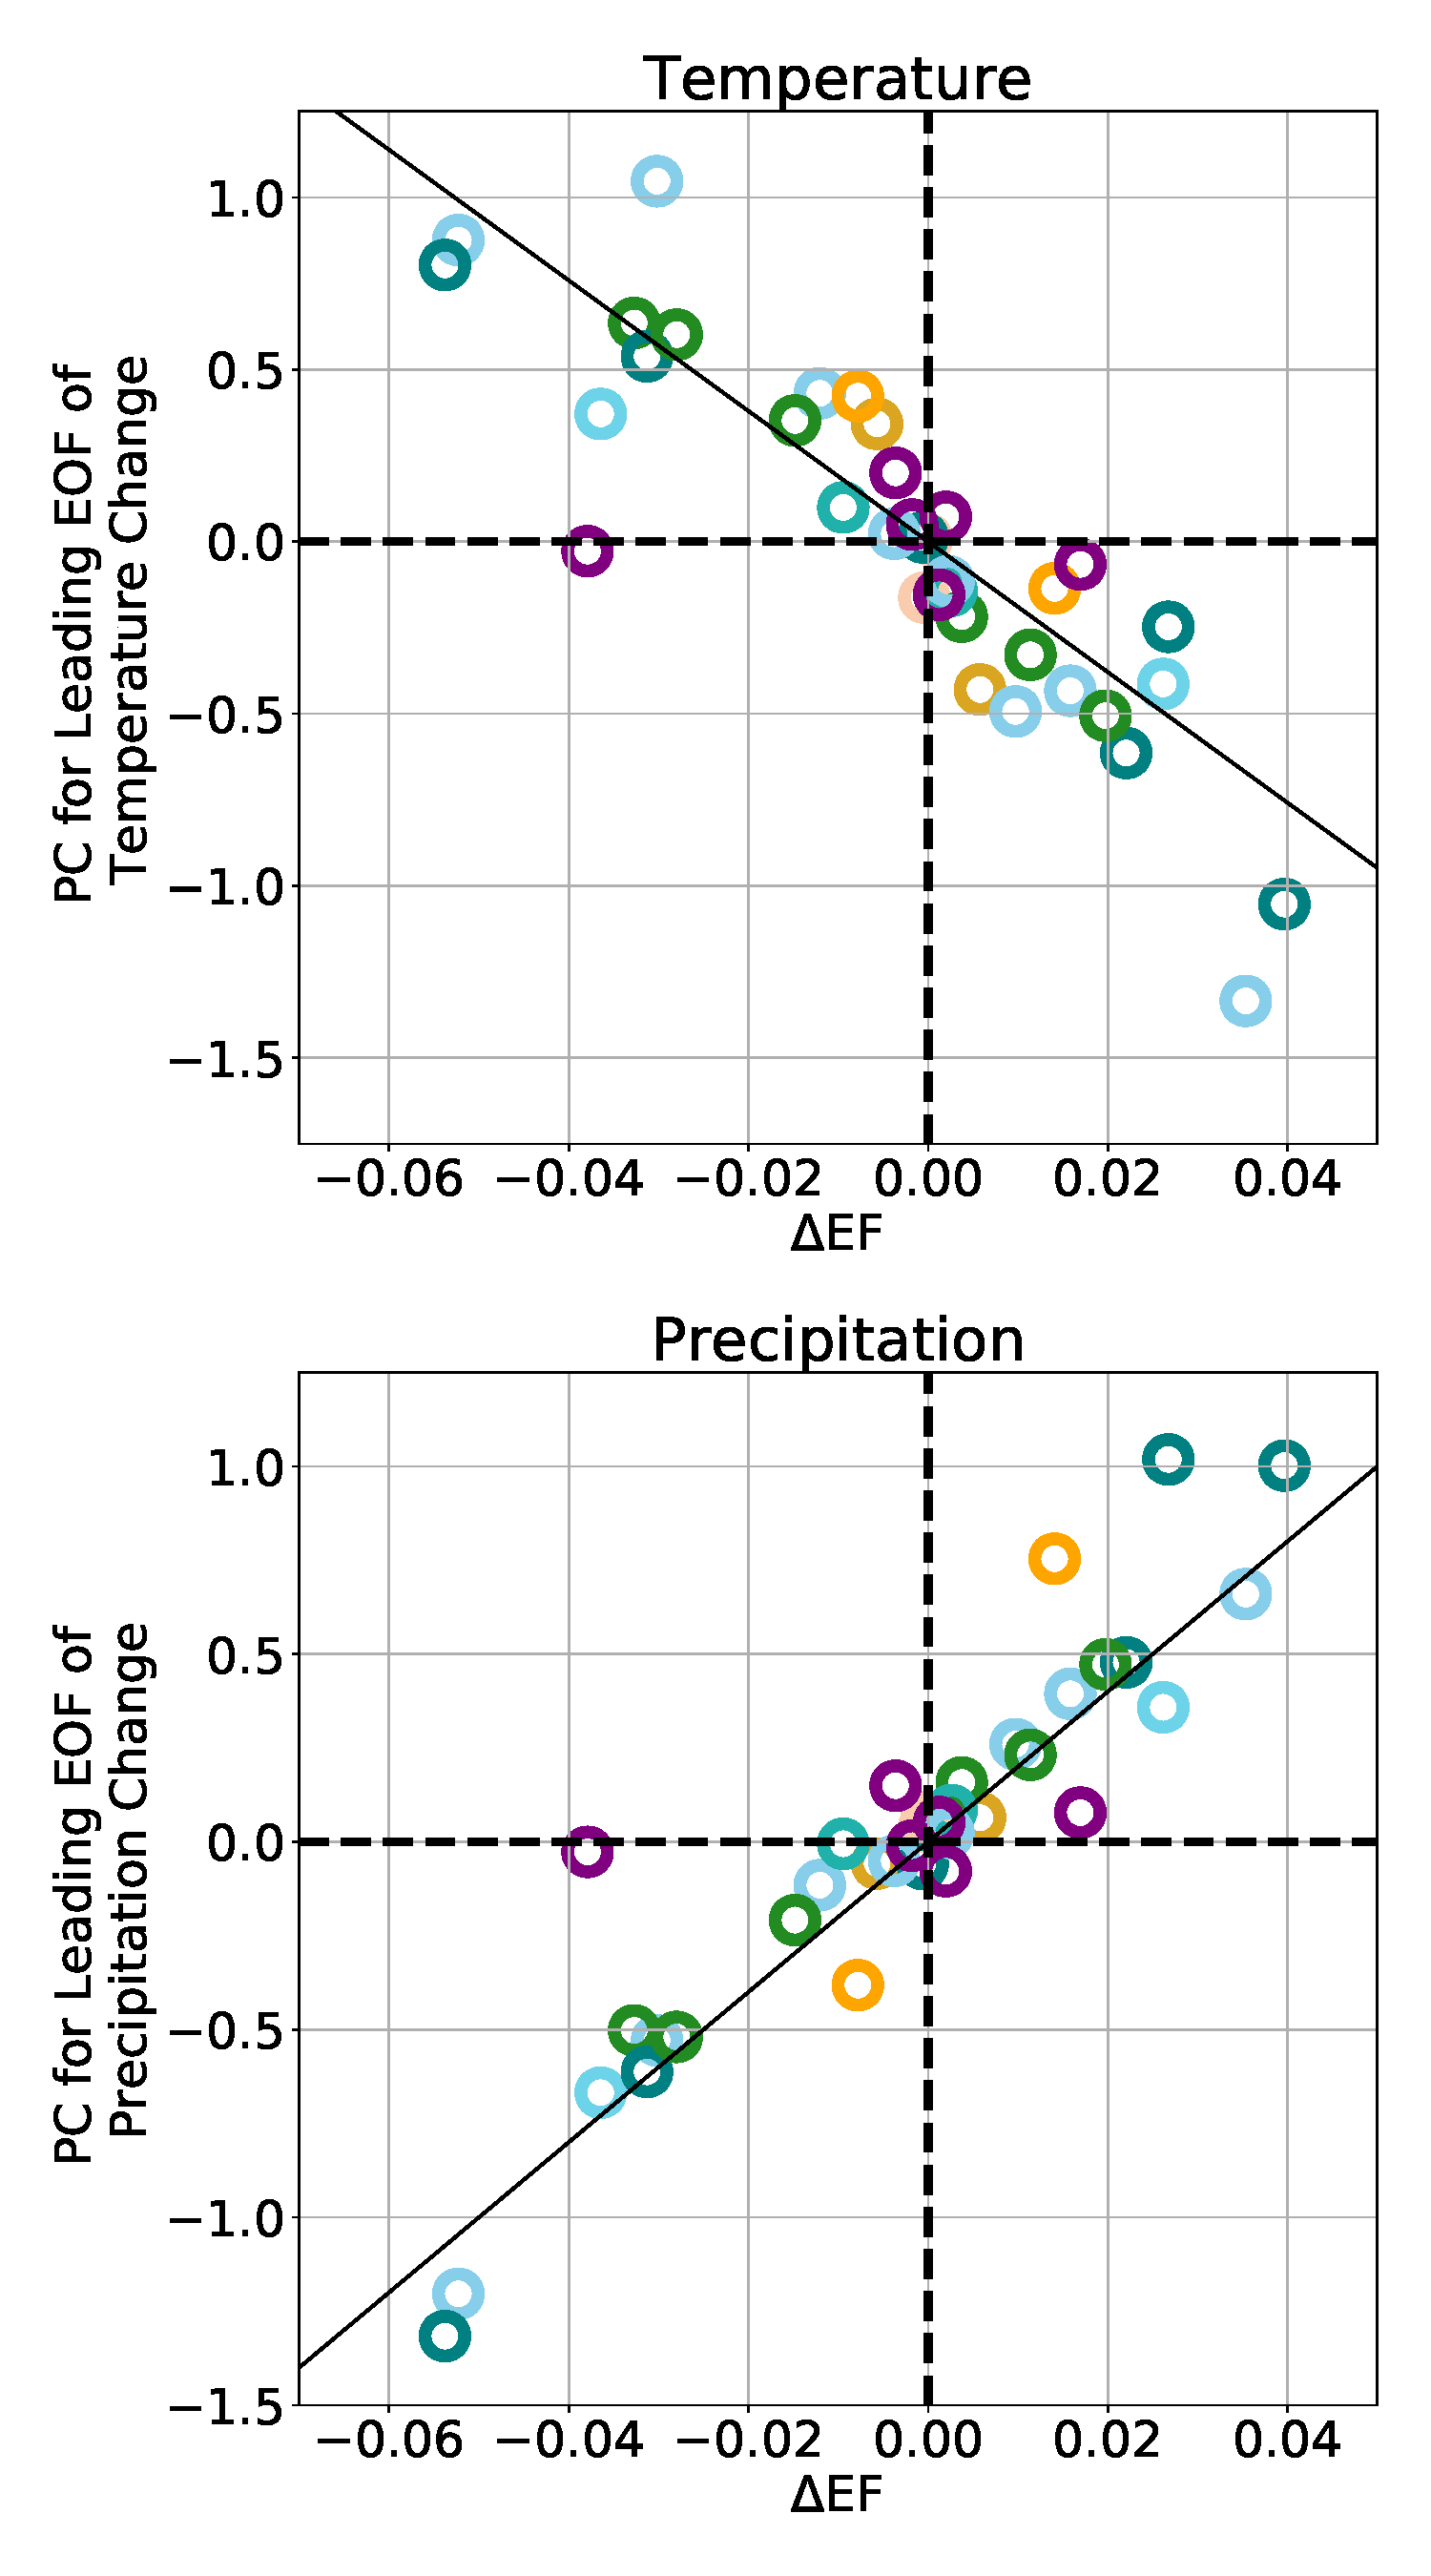
\includegraphics[width=0.75\textwidth]{writing/figs/Figure_S_EOF_vs_Temperature_and_Precipitation.pdf}
\caption{Correlation between change in global mean evaporative fraction (EF) and first principal components of temperature (top) and precipitation (bottom) change across the PPE. Colors indicate parameter category as in Figure 1.}
\label{fig:supp_EF_EOF_correlation}
\end{figure}

\begin{figure}[htb!]
\noindent\includegraphics[width=\textwidth]{writing/figs/Figure_S7.pdf}
\caption{Maps of annual mean land precipitation changes for each ensemble member, compared to the reference case with default parameterizations. Hatching indicates regions where the precipitation change was insignificant at the 0.05 significance level. The percentage of land with statistically significant temperature changes are shown in parentheses, and * indicates field significance.For each grid cell, we performed a two-tailed Student’s t-test to test whether the ensemble member mean (standard deviation calculated from the distribution from interannual variability in the ensemble member mean) was different from the default mean (standard deviation calculated from the distribution from interannual variability in the default mean). We test for field significance using Walker’s test.}
\label{fig:supp_maps_precip}
\end{figure}

\begin{figure}[htb!]
\noindent\includegraphics[width=\textwidth]{writing/figs/Figure_S7_withOcean.pdf}
\caption{Maps of annual mean precipitation changes for each ensemble member, including both land and ocean. Hatching and significance testing is as in Figure S7, but the title indicates the total percentage of the Earth surface (including land and ocean) with statistically significant temperature changes.}
\label{fig:supp_maps_precip_landAndOcean}
\end{figure}

\begin{figure}[htb!]
\noindent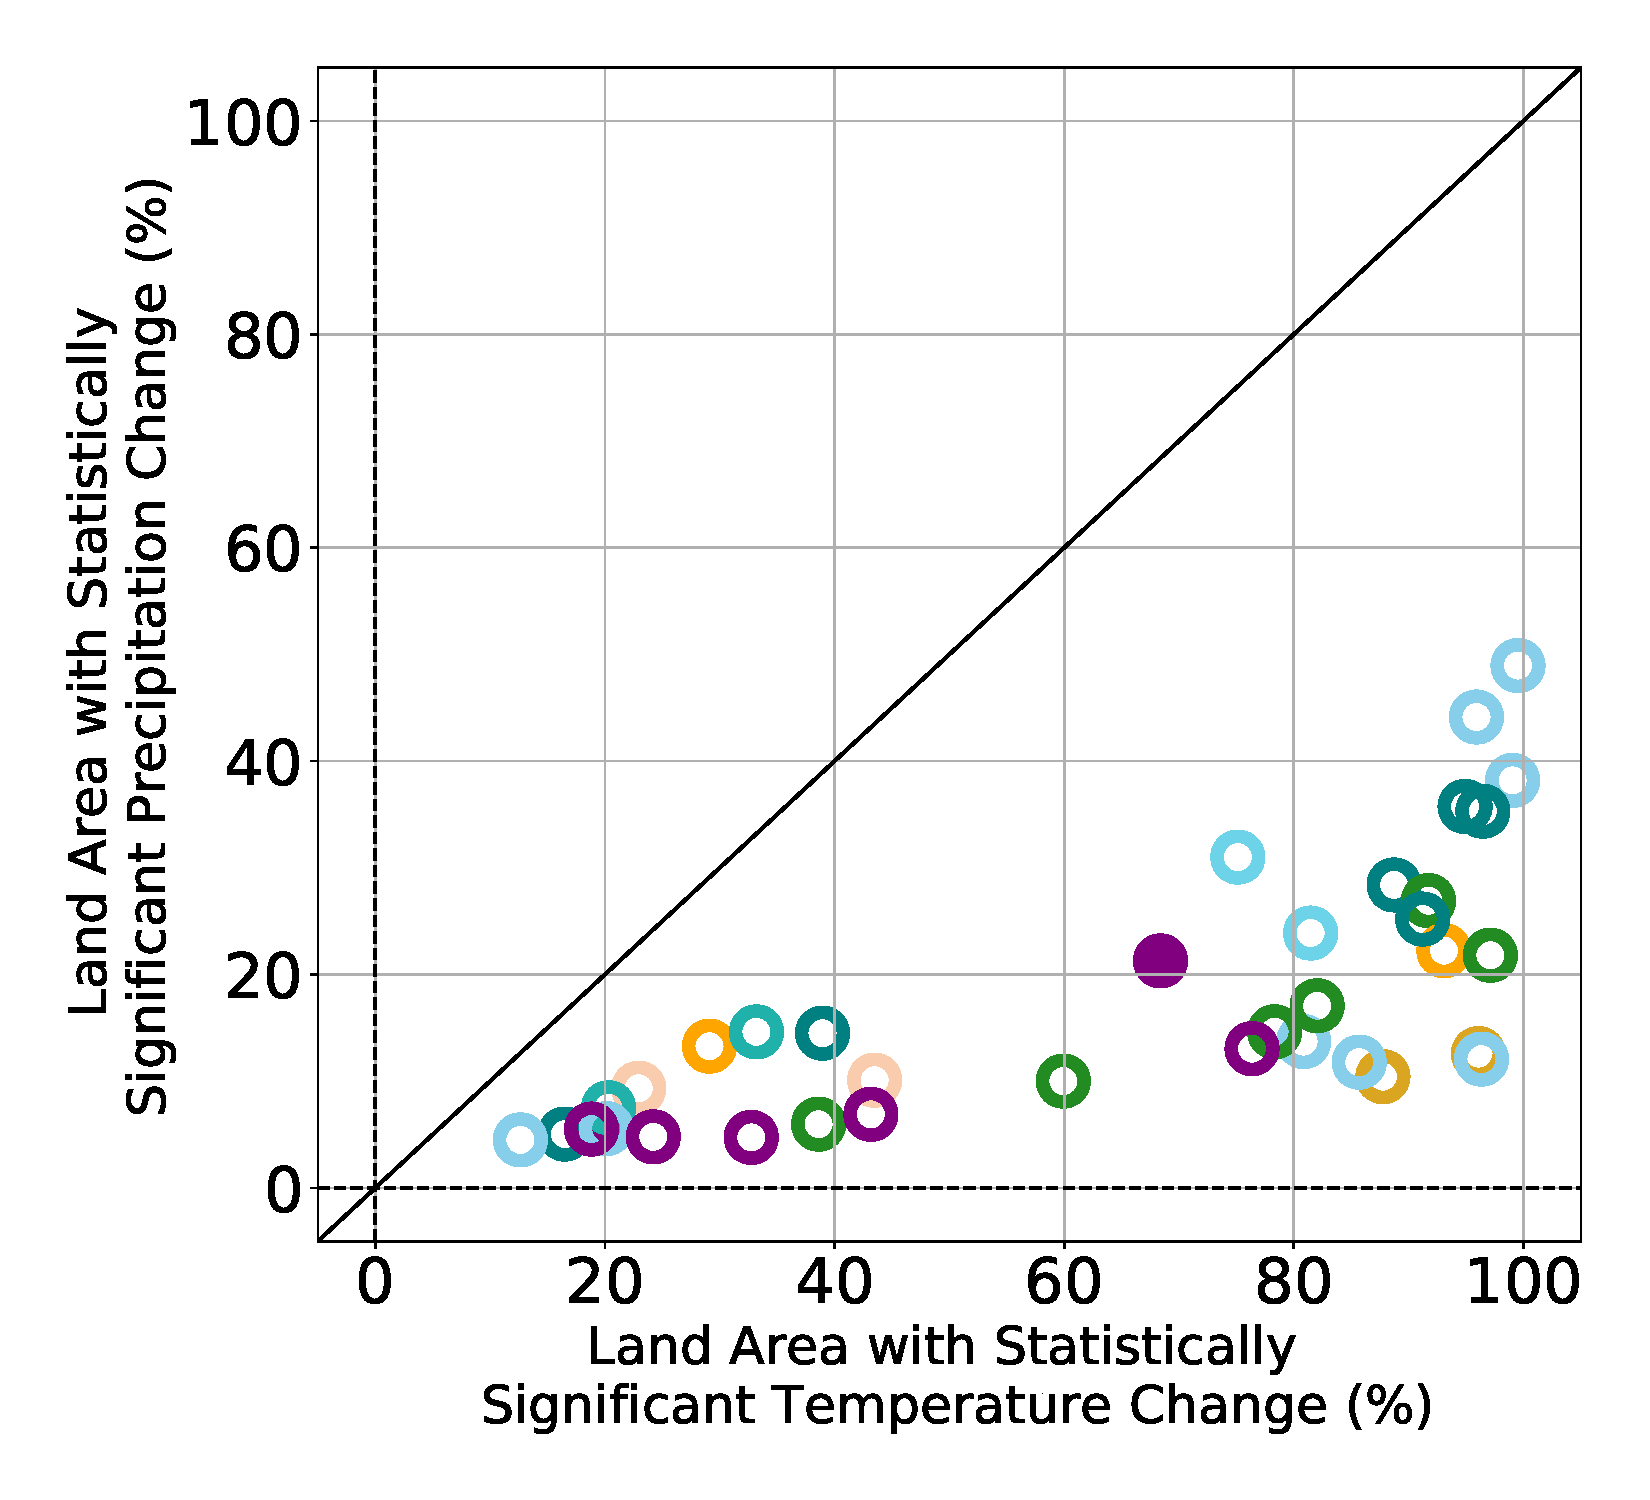
\includegraphics[width=\textwidth]{writing/figs/Figure_S8.pdf}
\caption{Percentage of land area with statistically significant temperature vs. precipitation changes for each ensemble member in the PPE. Ensemble members are colored by parameter category, as in Figure 1. Zetamaxstable is indicated with a filled circle because it is a frequent outlier.}
\label{fig:supp_pct_stat_sig_land}
\end{figure}

\begin{figure}[htb!]
\noindent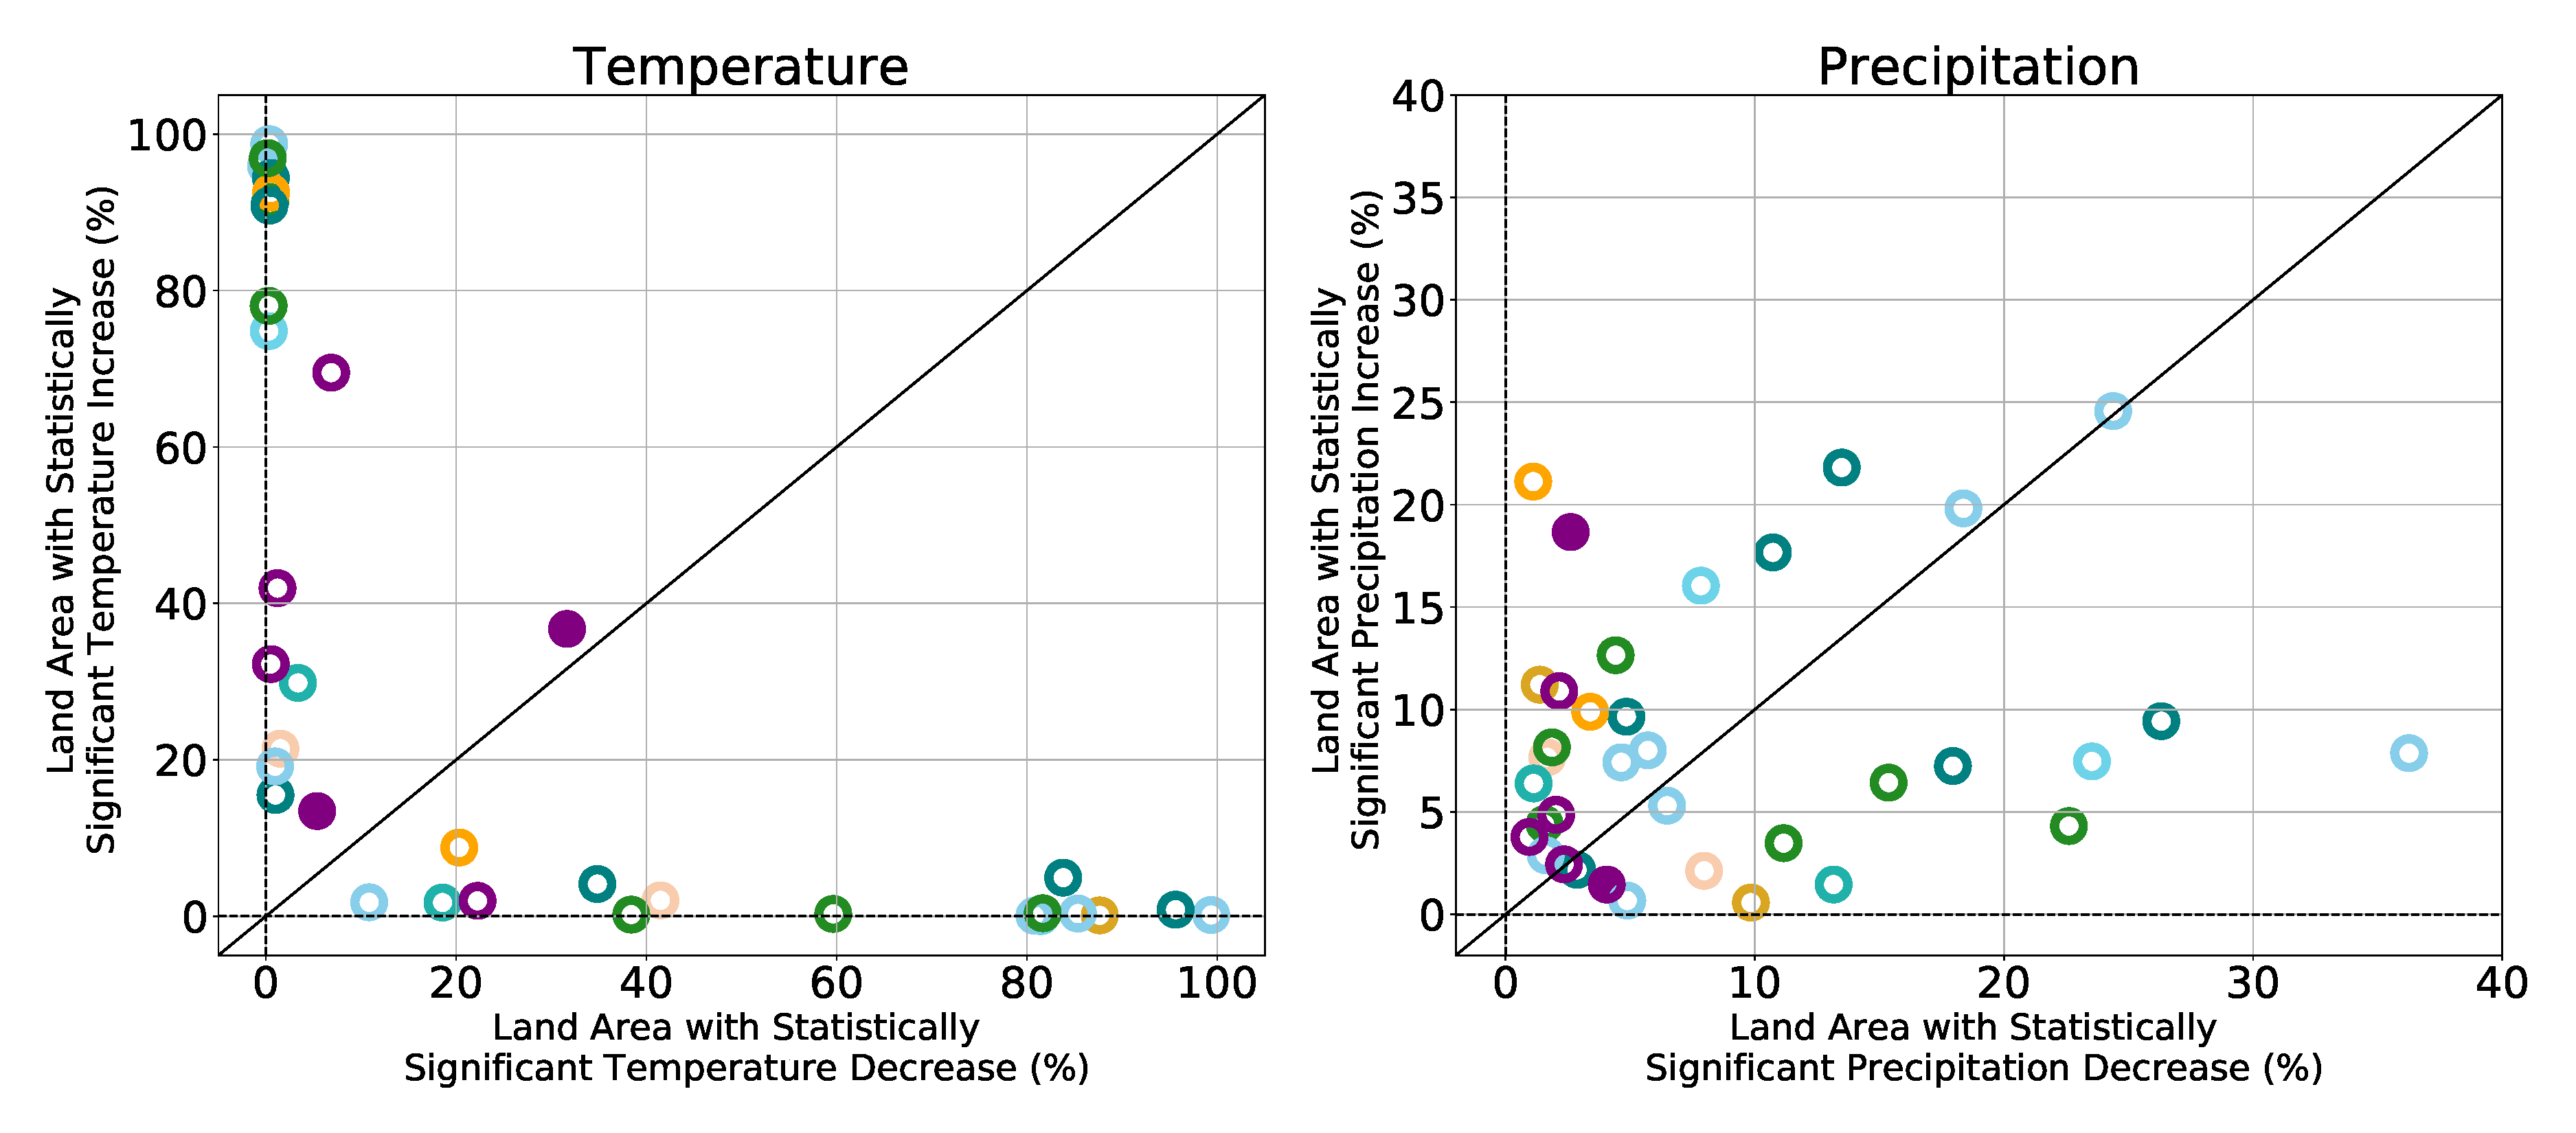
\includegraphics[width=\textwidth]{writing/figs/Figure_S9_Percentage_Significant_Sign_Change.pdf}
\caption{Sign of change of statistically significant mean climate changes across the PPE. Percent of land area experiencing statistically significant decreases vs. increases in temperature (left) and precipitation (right) for each PPE ensemble member. Ensemble members are colored by parameter category, as in Figure 1. We note that one parameter (\mintinline{Fortran}{zetamaxstable}) drove statistically significant temperature changes of opposite sign across 63$\%$ of land area, which canceled each other out in the global mean resulting in a minimal global mean land temperature change (Figure S\ref{fig:supp_coupled_Ts_land_maps}) - this parameter is indicated with a filled circle because it is a frequent outlier.}
\label{fig:supp_pct_stat_sig}
\end{figure}

\begin{figure}[htb!]
\noindent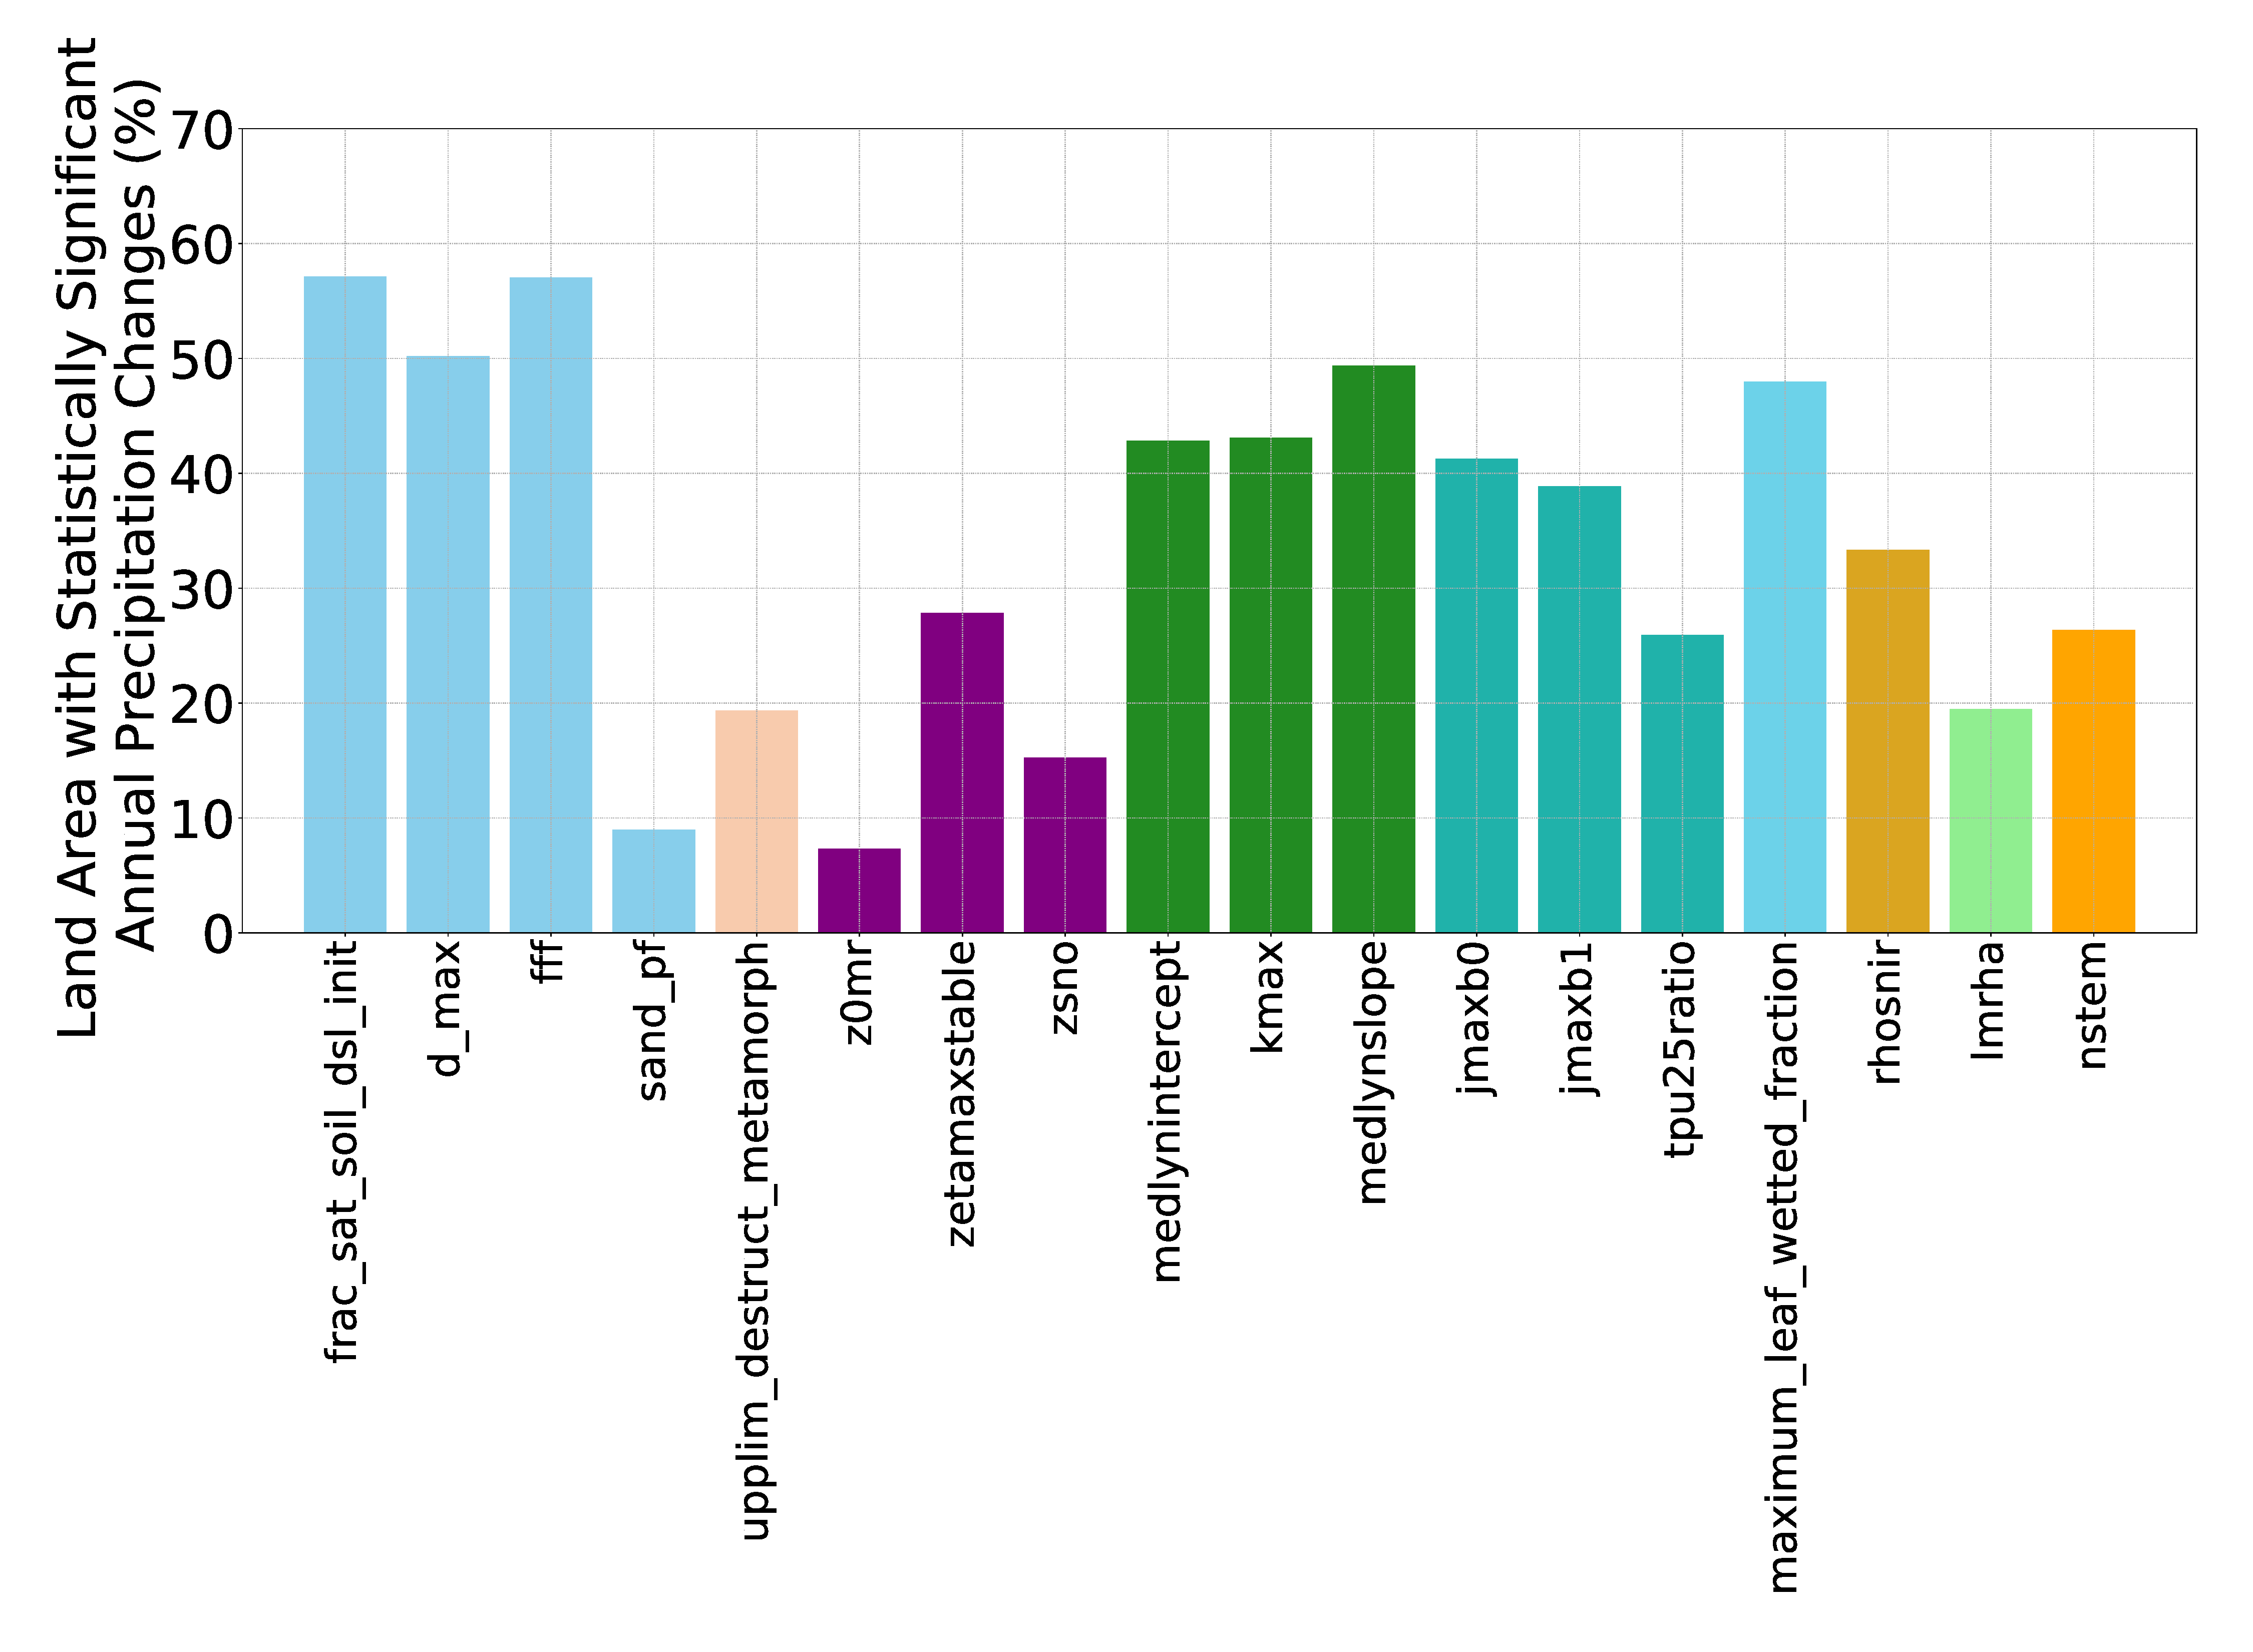
\includegraphics[width=\textwidth]{writing/figs/Figure_S_Precip_Change_Significance_by_Parameter.pdf}
\caption{Percentage of global land area that experiences statistically significant changes in annual mean precipitation due to perturbations in each parameter. For each land grid cell, we performed a two-tailed Student’s t-test to test whether the parameter maximum simulation was different from the parameter minimum simulation.}
\label{fig:supp_precip_significance_changes}
\end{figure}

\begin{figure}[htb!]
\noindent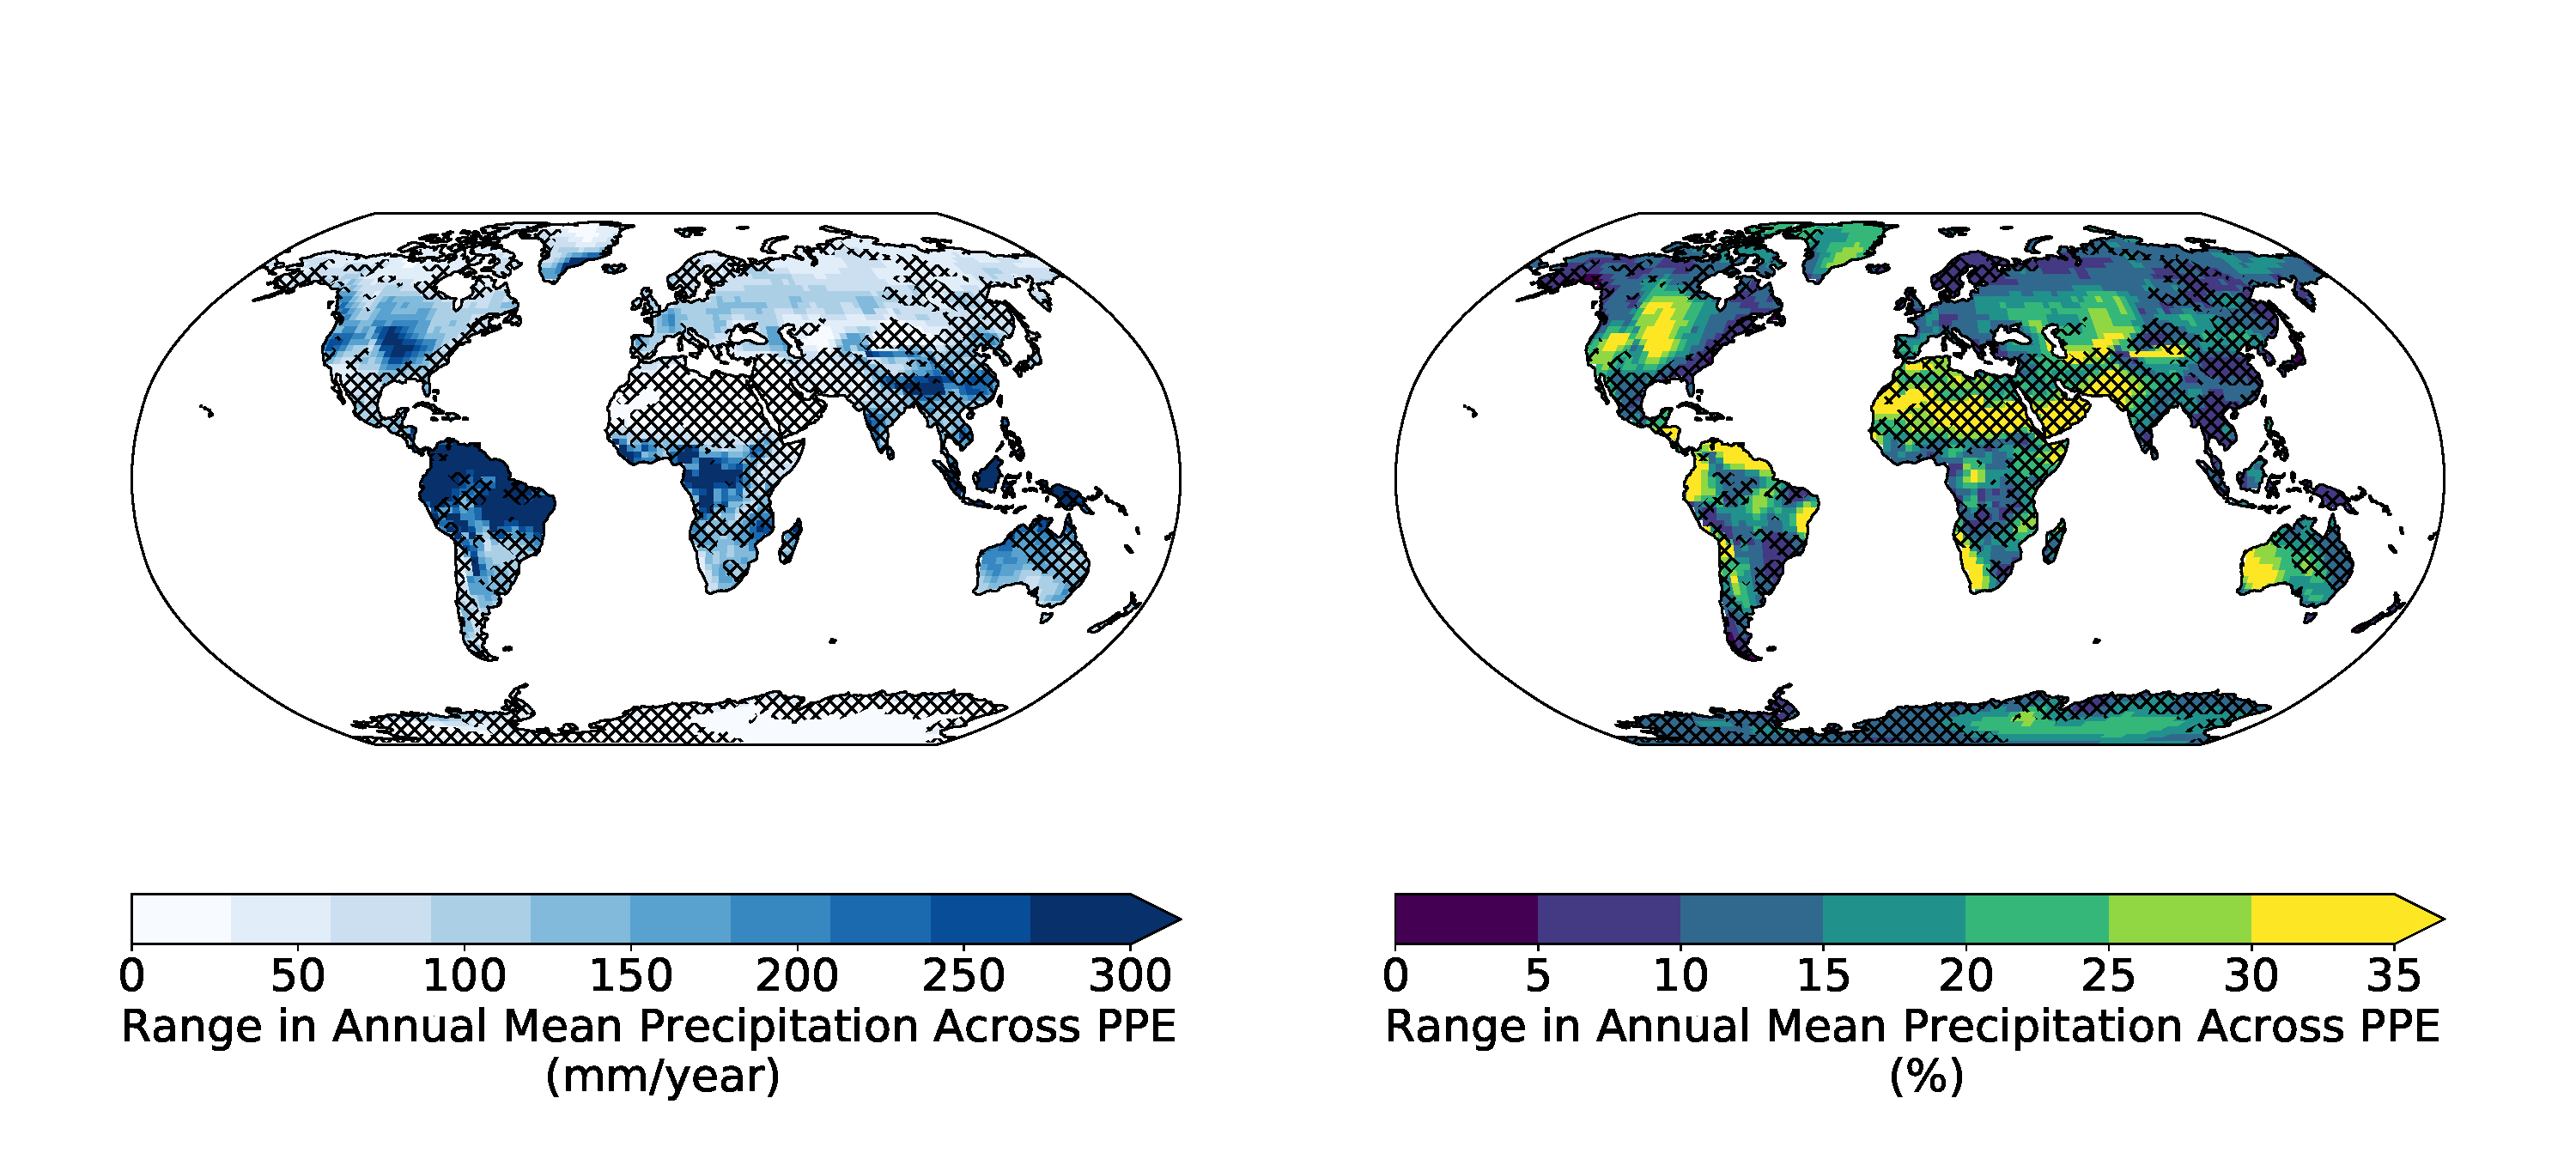
\includegraphics[width=\textwidth]{writing/figs/PRECT_range_absolute_change.pdf}
\caption{Range in annual mean precipitation changes across the PPE, on an absolute basis (left) and as a percentage of the default precipitation (right). Hatching indicates regions where annual mean precipitation changes were statistically insignificant for five or more ensemble members.
}
\label{fig:supp_precip_range}
\end{figure}

\begin{figure}[htb!]
\noindent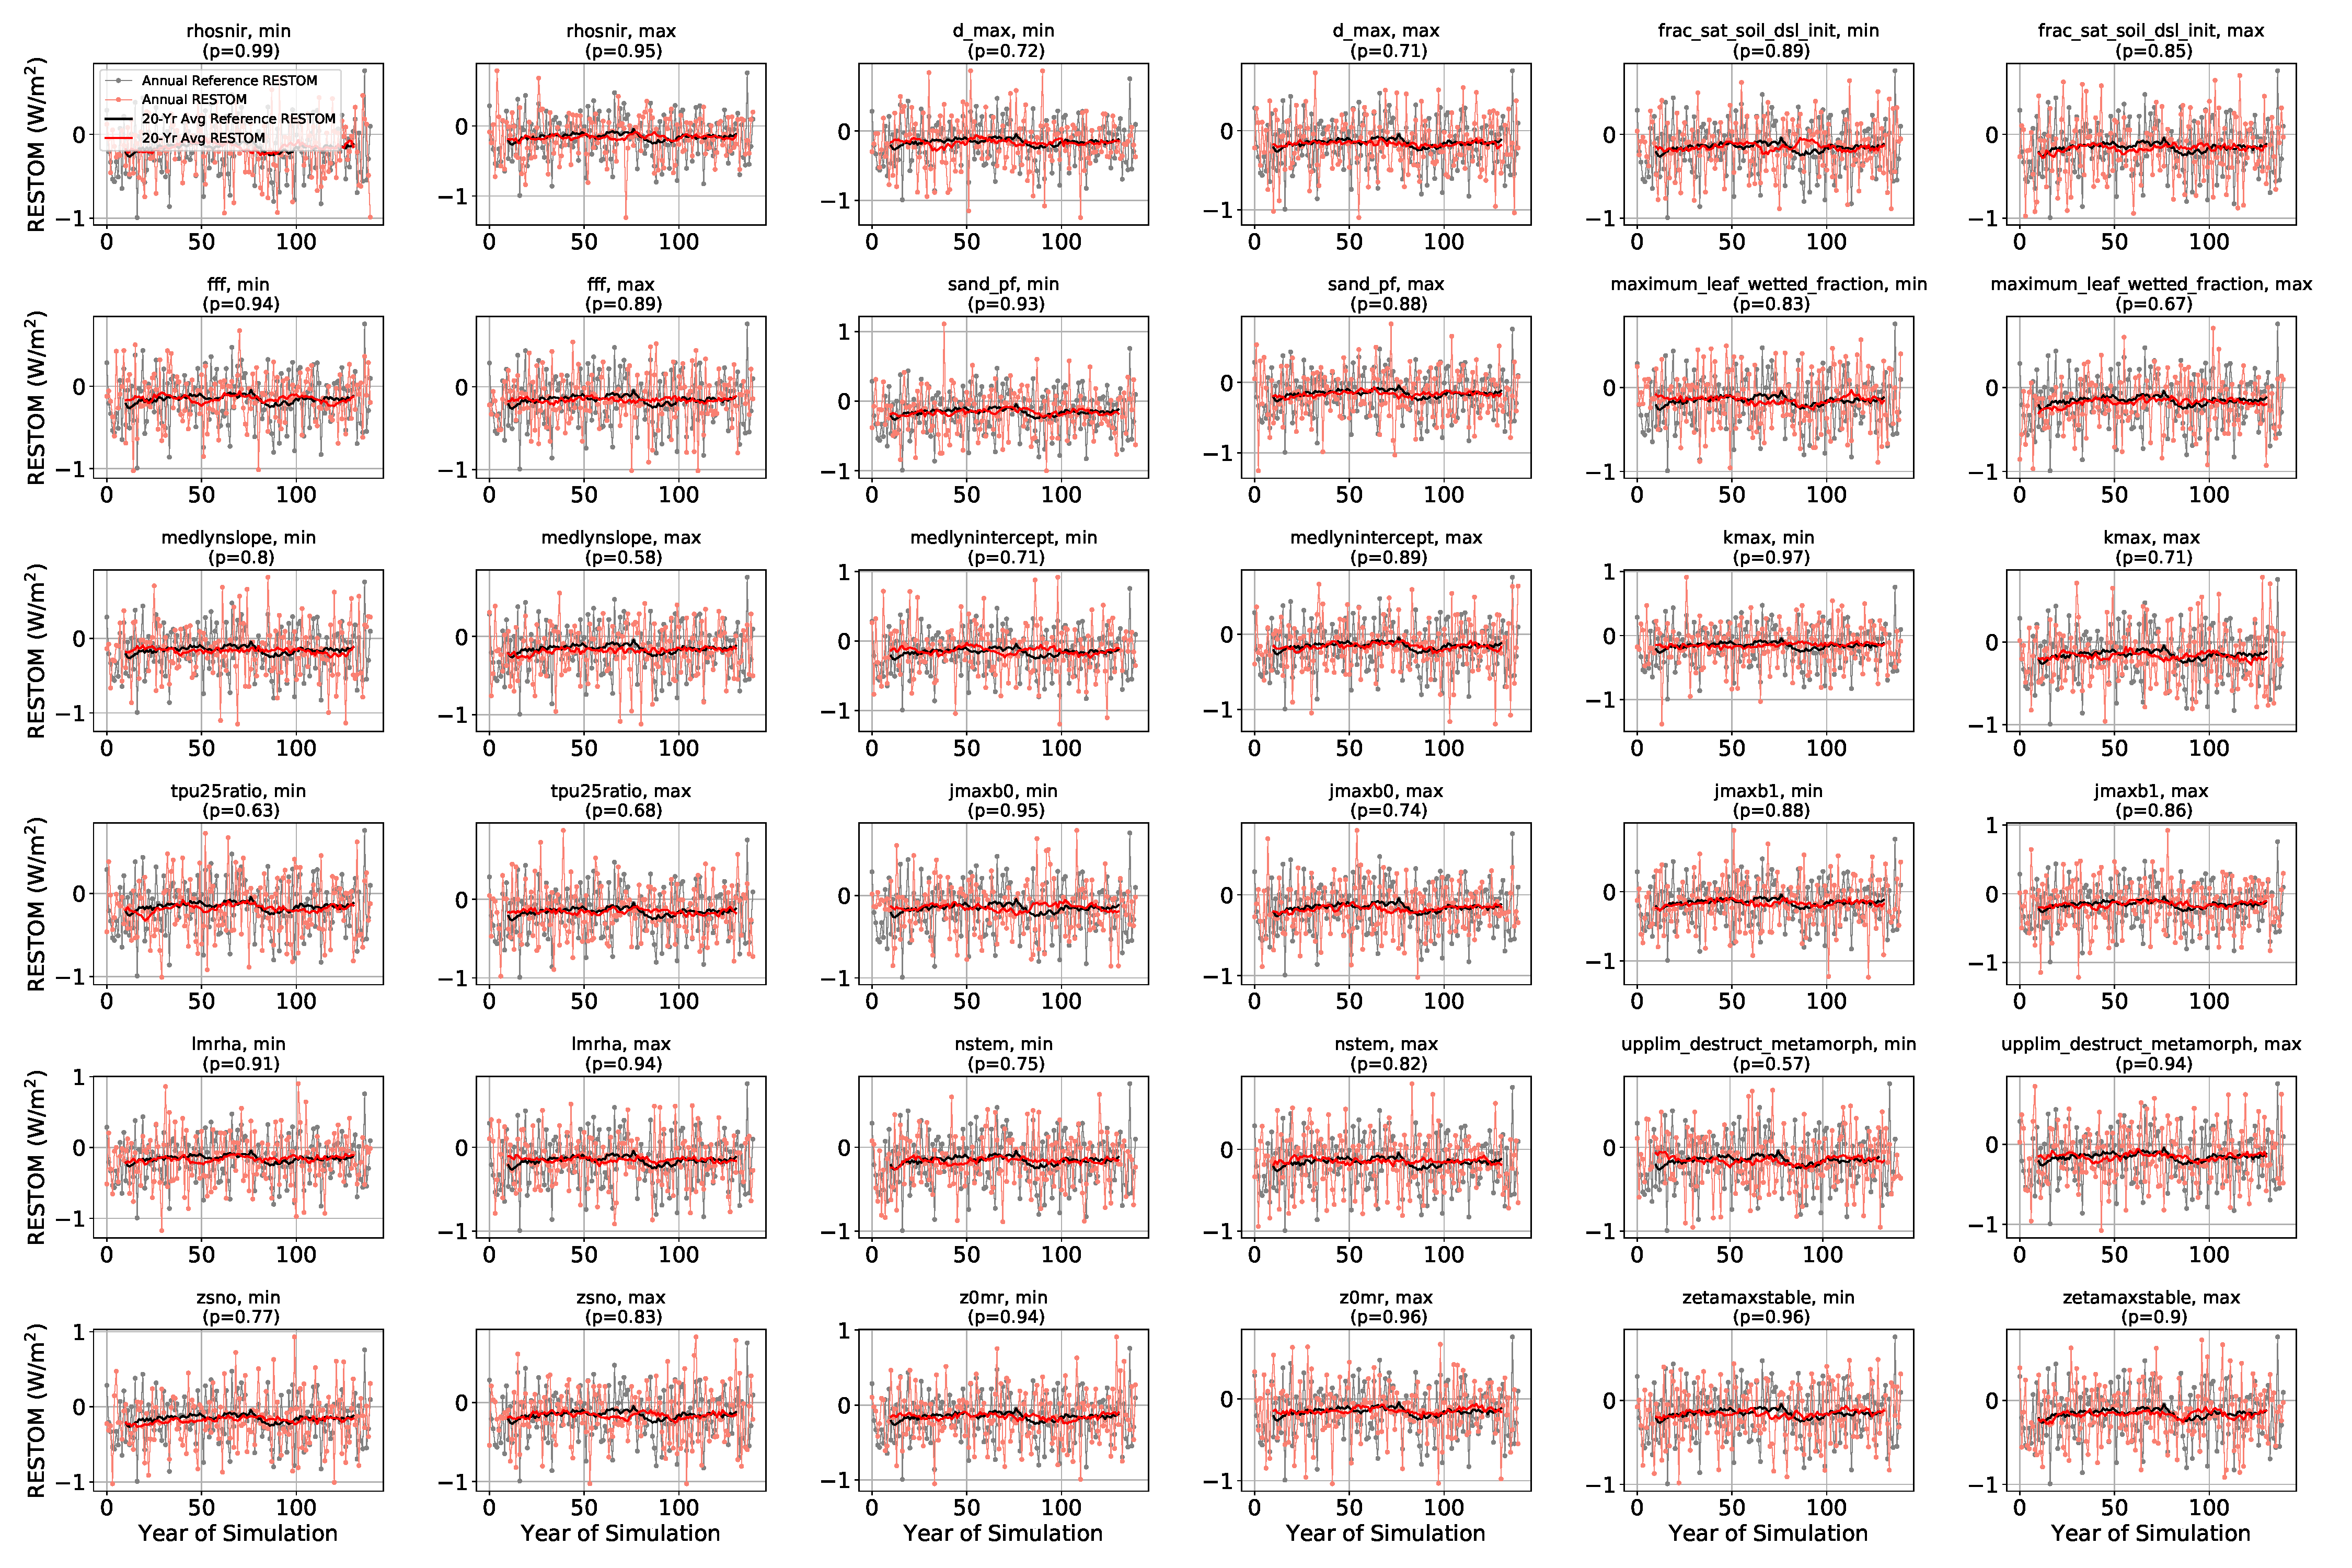
\includegraphics[width=\textwidth]
{writing/figs/Figure_S_Minimal_RESTOM_differences.pdf}
\caption{Time series of the net radiative flux at the top of the model (RESTOM), as calculated from the net solar flux at top of model (FSNT) minus the net longwave flux at top of model (FLNT). The average RESTOM for the last 100 years of the reference case is -0.15 W$/$m$^2$. RESTOM varied minimally across the ensemble ($\sigma$=0.010 W/m$^2$), and was not statistically significantly different from the reference case for any ensemble member. Significance was tested using two-tailed Student’s t-test on the  time series of annual mean RESTOM.}
\label{fig:supp_TOA_energy_balance}
\end{figure}

\begin{figure}[htb!]
\noindent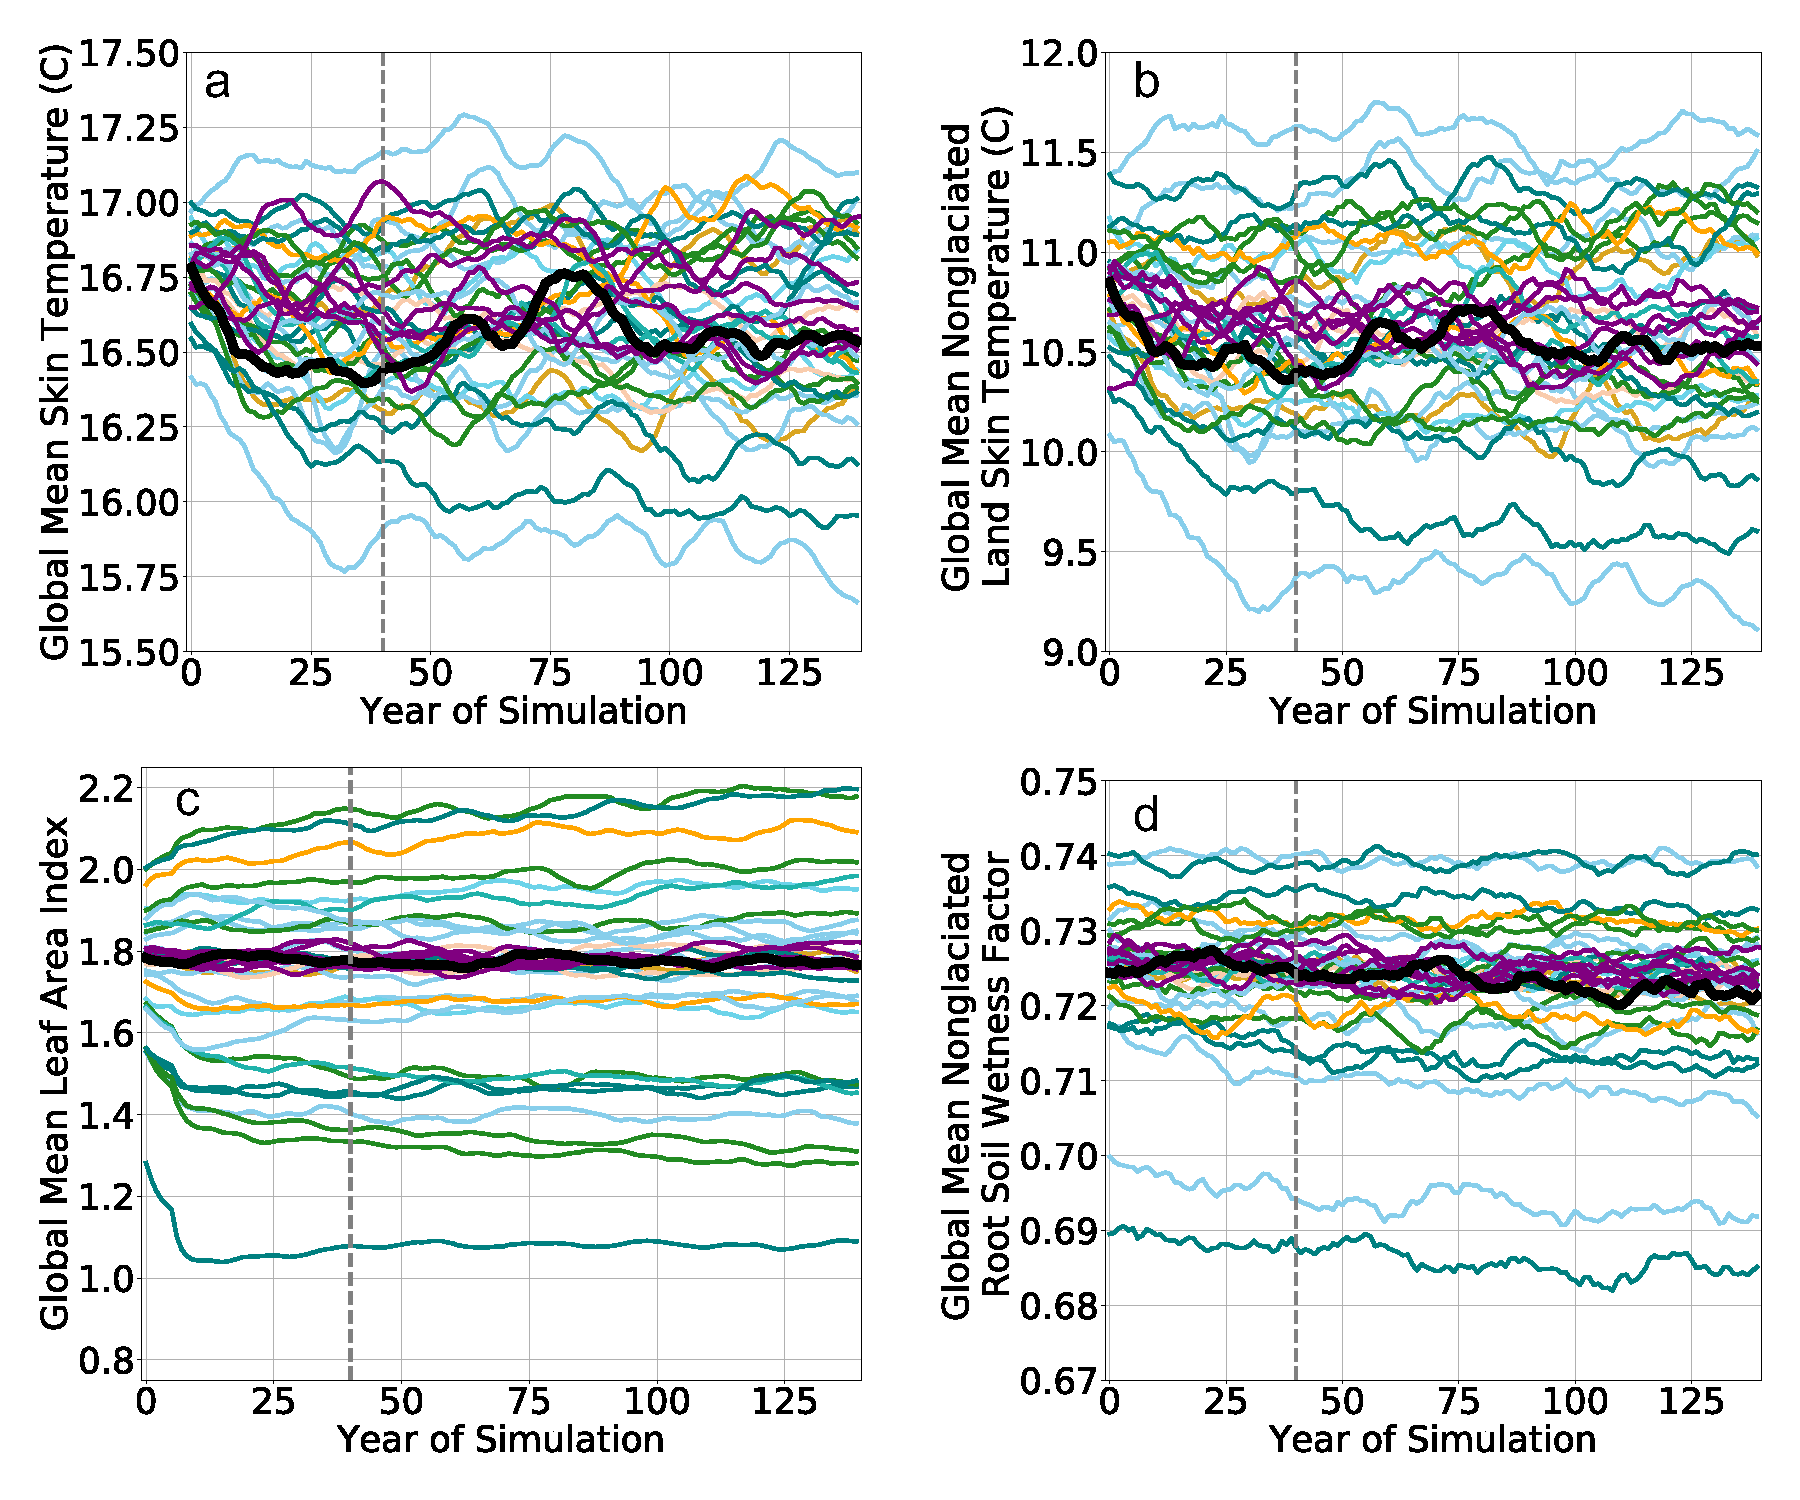
\includegraphics[width=\textwidth]{writing/figs/Figure_S_SpinUp.pdf}
\caption{Time series of annual mean (a) global temperature, (b) global land temperature, (c) global leaf area index, and (d) global root zone soil wetness factor (where 1 indicates no water stress) for each ensemble member of the PPE. The black line indicates the reference simulations, and ensemble members are colored by parameter category as in Figure 1. The first 40 years of each simulation (denoted by dashed vertical line) were discarded as spin up. Data in panels (c) and (d) are averaged over non-glaciated land only.}
\label{fig:supp_spinup}
\end{figure}

%\end{document}

%\section*{Supplemental Tables}

\captionsetup[table]{format=cancaption,labelformat=cancaptionlabel}
 \begin{table}[htb!]
 \centering
\noindent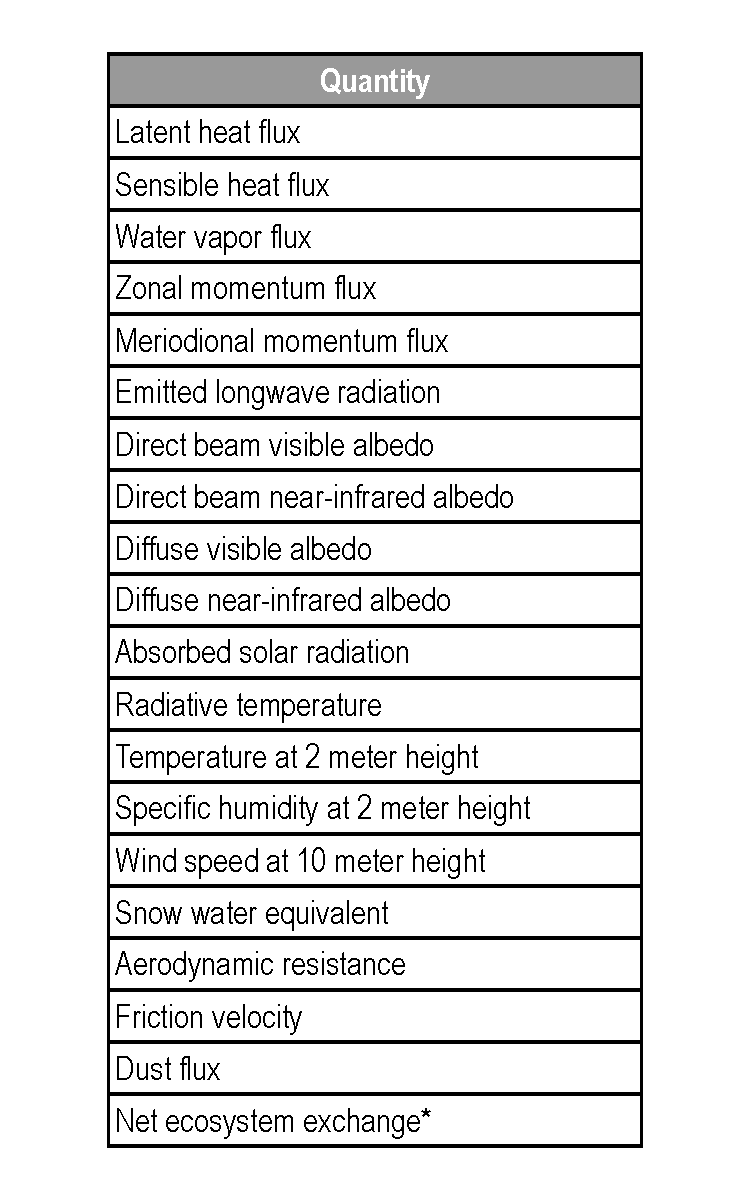
\includegraphics[width=0.5\textwidth]{writing/figs/Table_Land2Atm_Quantities.pdf}
  \caption{Quantities that the land model passes to the atmosphere in CESM2. \footnotesize{Note that net ecosystem exchange does not impact the atmosphere in our experimental design because our experimental design held atmospheric CO$_2$ concentrations fixed.}}
 \label{table:metrics_of_impact}
 \end{table}

\begin{table}[htb!]
\noindent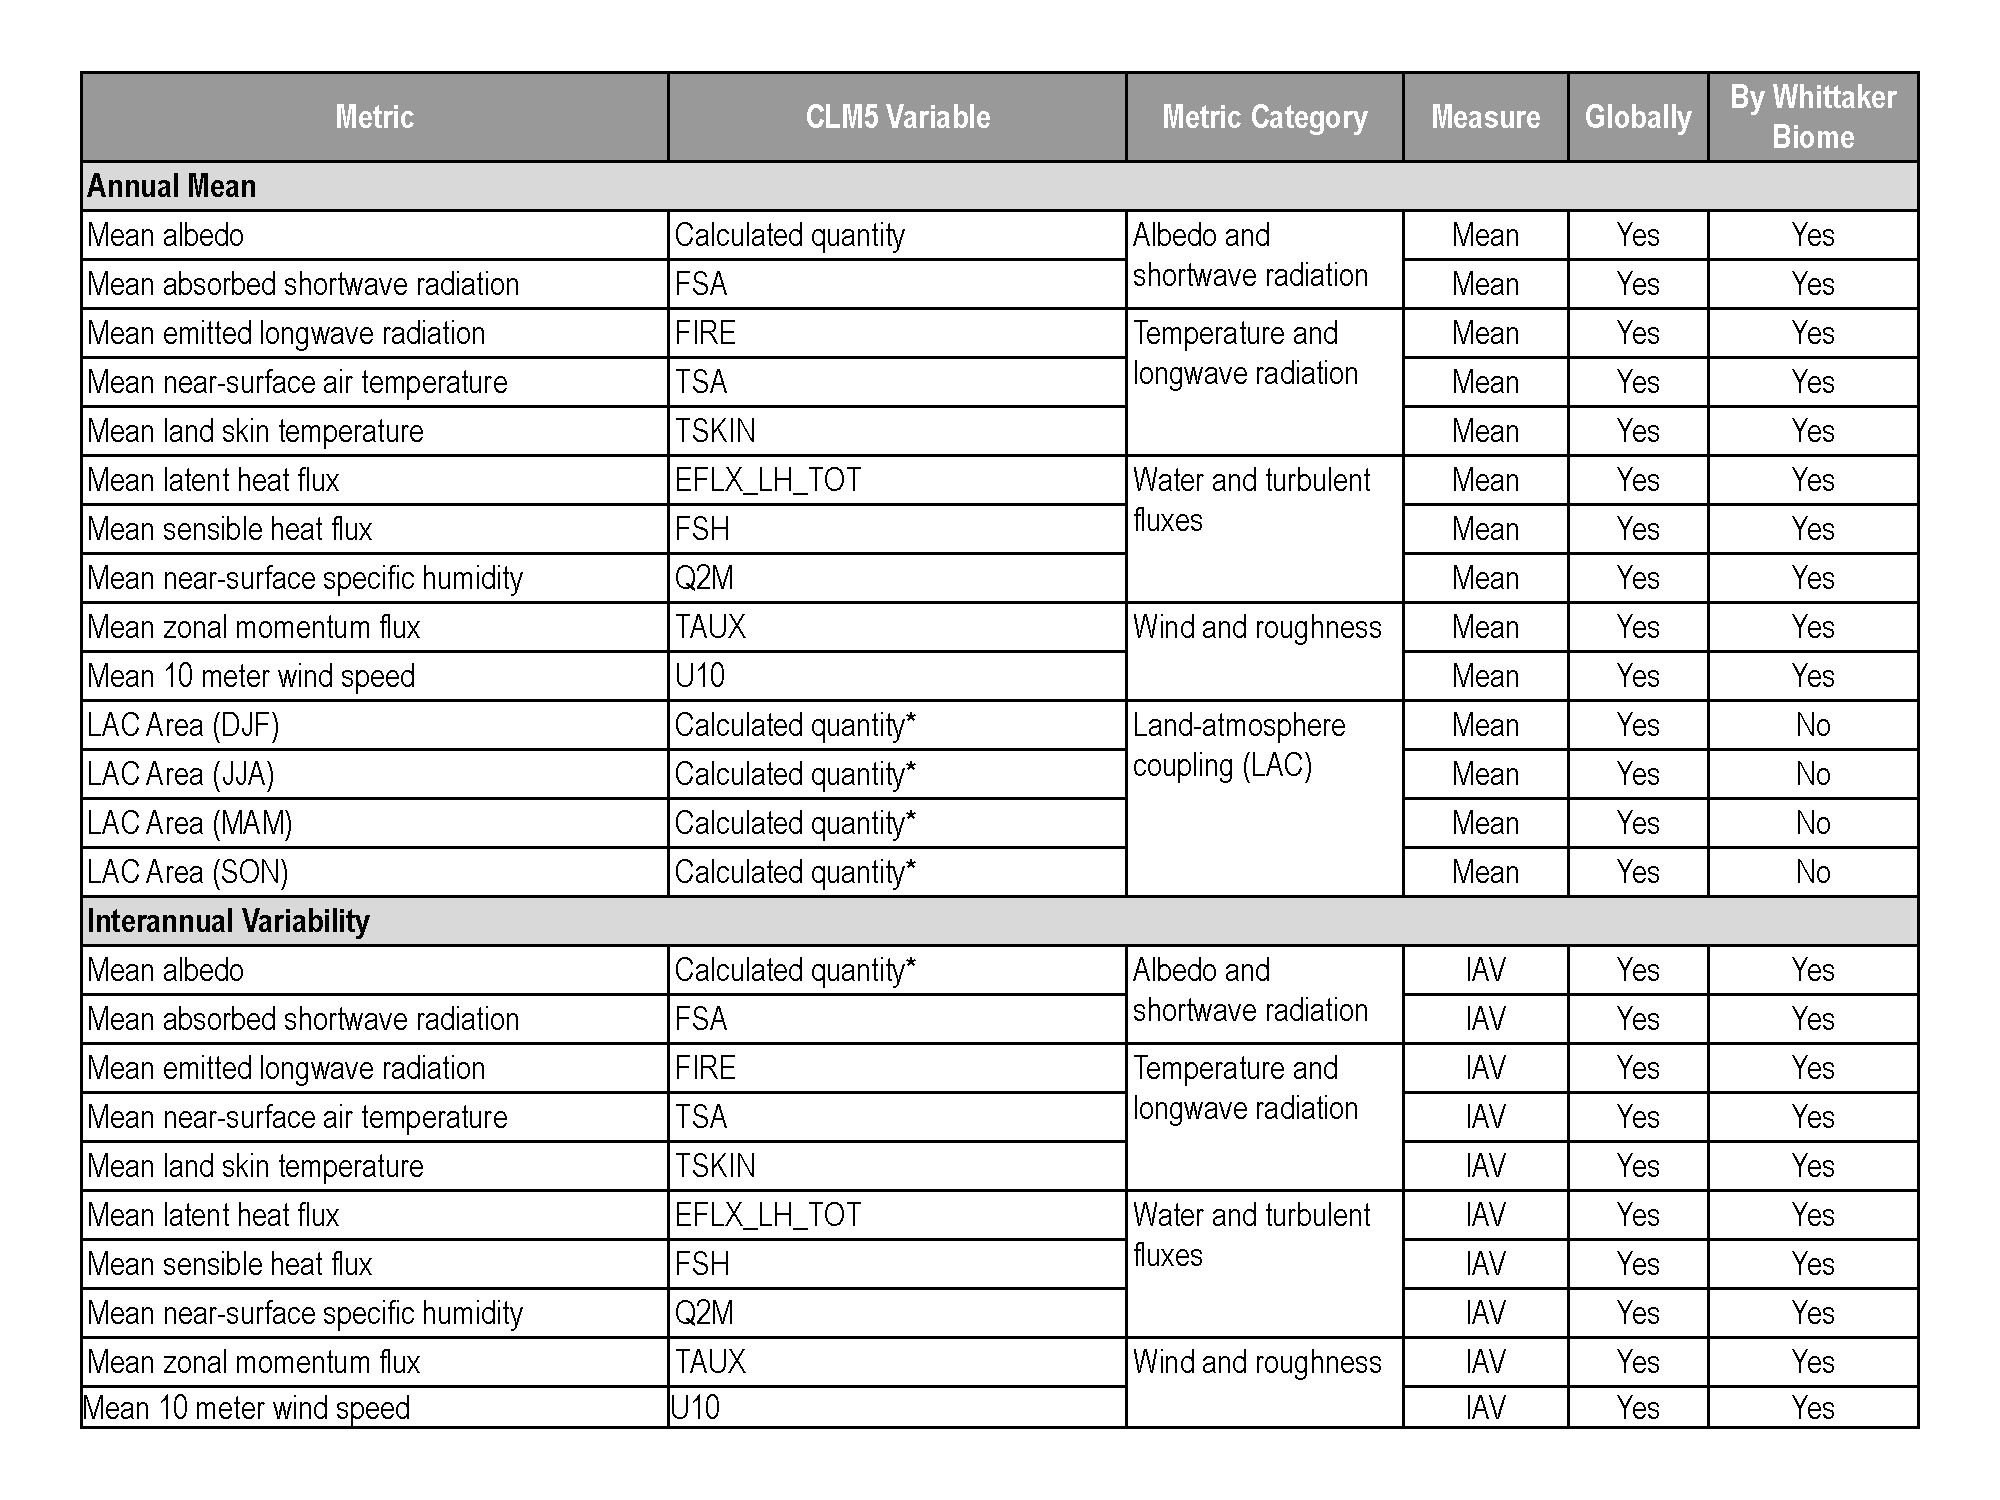
\includegraphics[width=\textwidth]{writing/figs/Table_Quantities_Used_In_Parameter_Selection.pdf}
  \caption{Metrics for evaluating parameter impact on land-to-atmosphere fluxes.}
 \label{table:land2atm_fluxes}
 \end{table}

 \captionsetup[table]{format=cancaption,labelformat=cancaptionlabel}
 \begin{table}[htb!]
 \centering
\noindent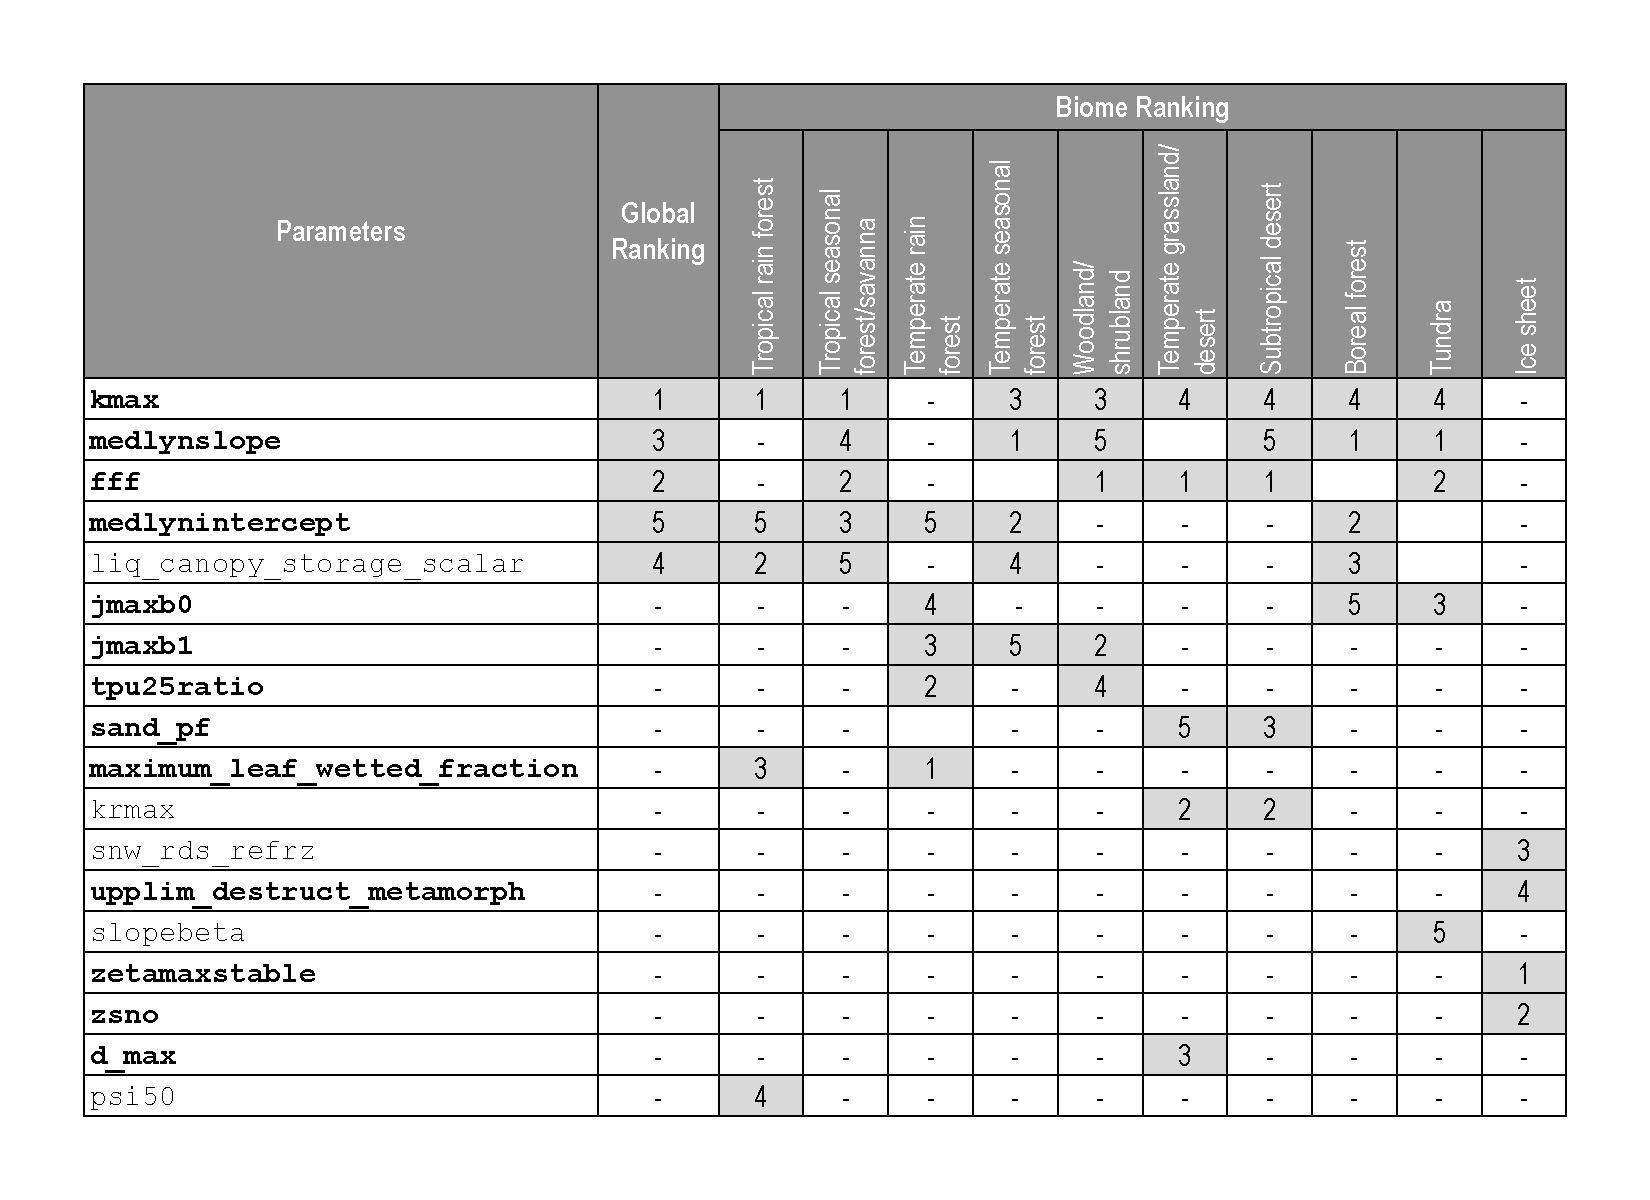
\includegraphics[width=\textwidth]{writing/figs/Table_Example_LH_Flux_Rankings.pdf}
  \caption{Example of parameter rankings in terms of their impact on mean latent heat flux, globally and for Whittaker biomes. Rankings are only shown if the parameter was ranked in the top 5. Bolded parameters were included in our PPE.}
 \label{table:LH_example_rankings}
 \end{table}

\begin{table}[htb!]
\noindent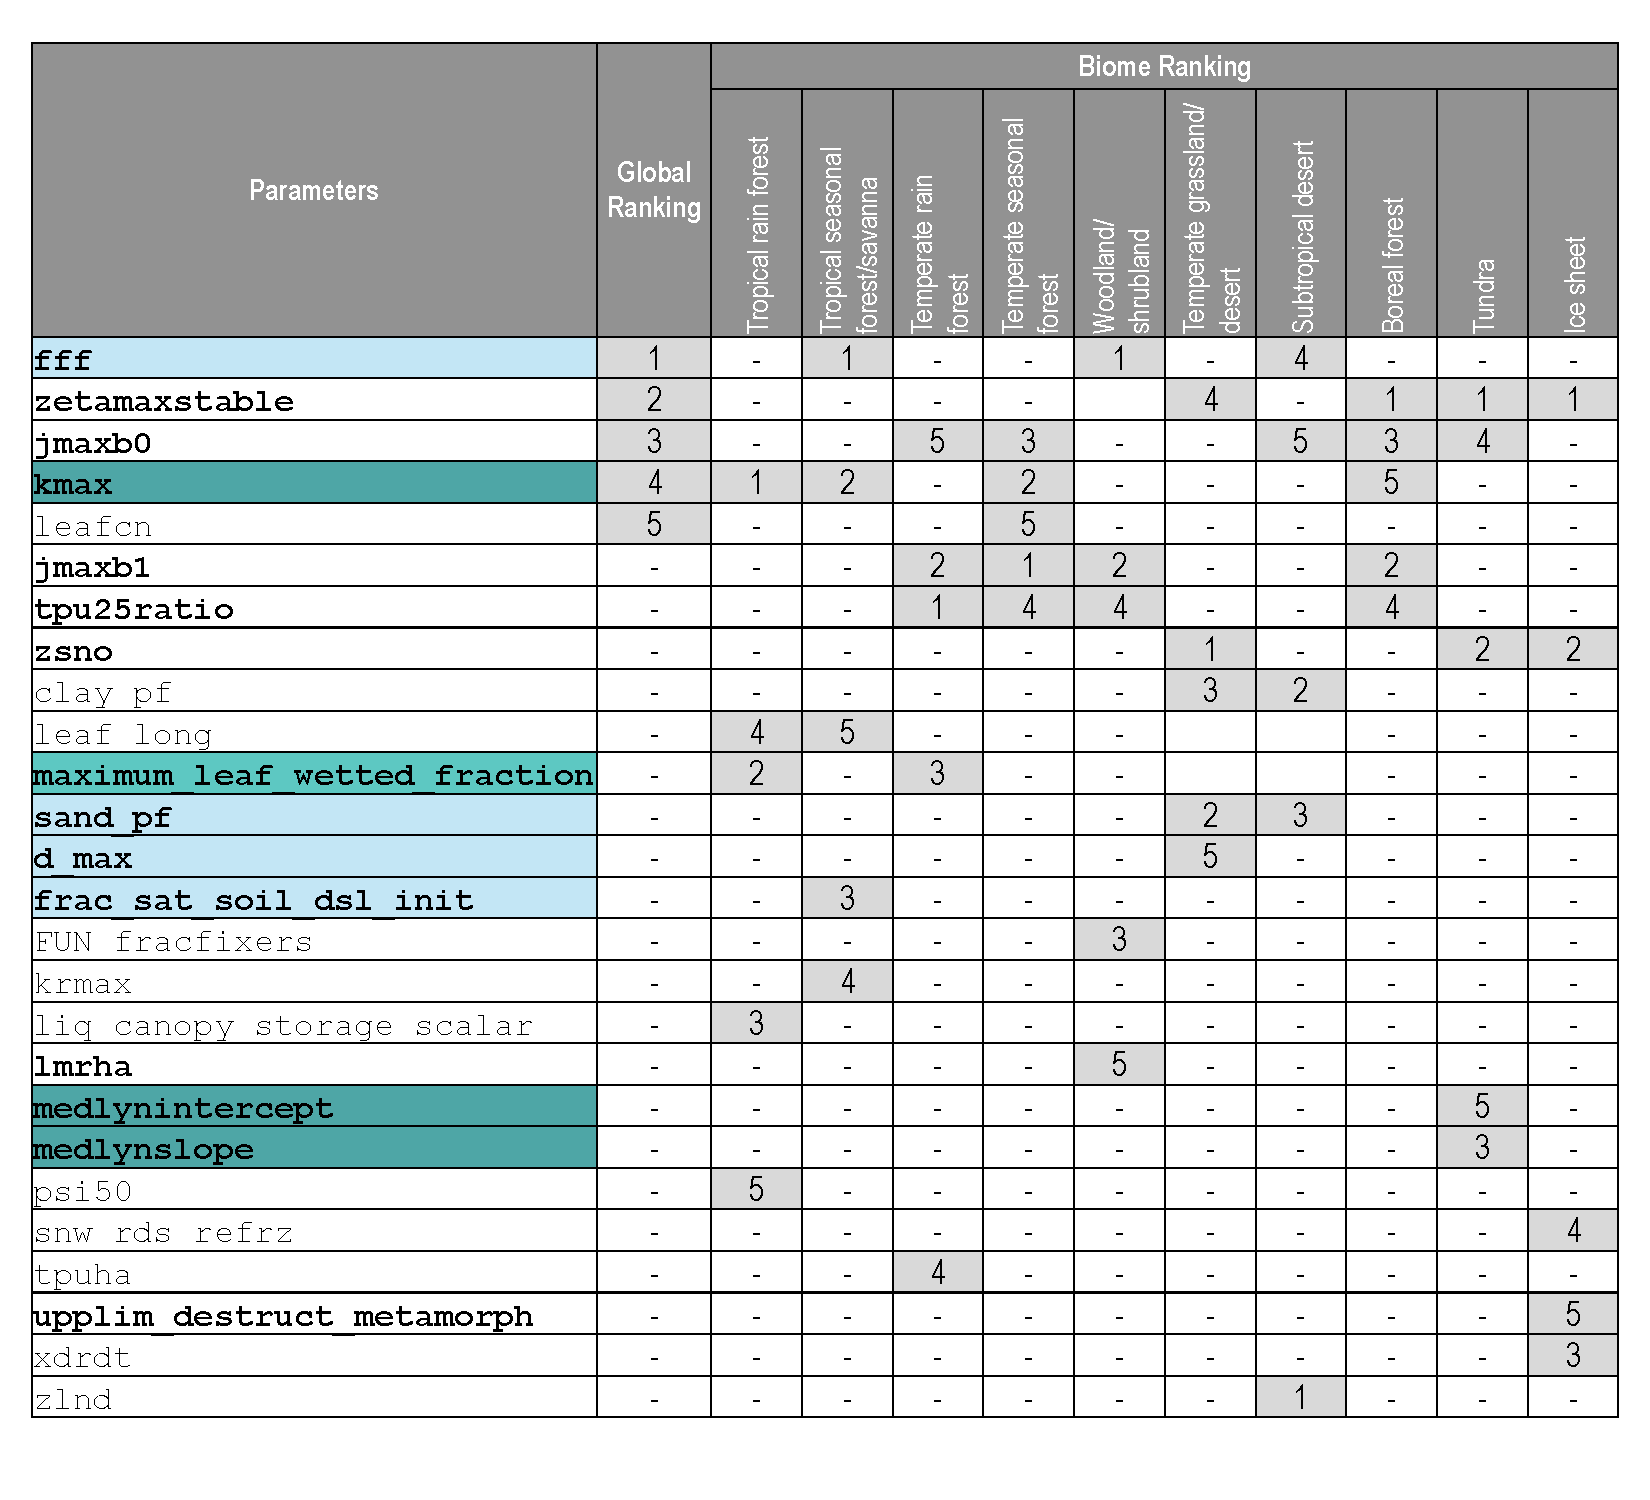
\includegraphics[width=\textwidth]{writing/figs/Table_Example_TSKIN_Rankings.pdf}
\caption{Rankings of parameters with the largest land surface temperature change in the land-only CLM5-PPE, globally and for Whittaker biomes. Rankings are only shown if the parameter was ranked in the top 5. Bolded parameters were included in our PPE, and parameters relating to soil hydrology, stomatal conductance and plant water use, and canopy evaporation are highlighted.}
\label{table:supp_param_rankings}
\end{table}

\begin{sidewaystable}
%\hspace*{-1.1in}
\noindent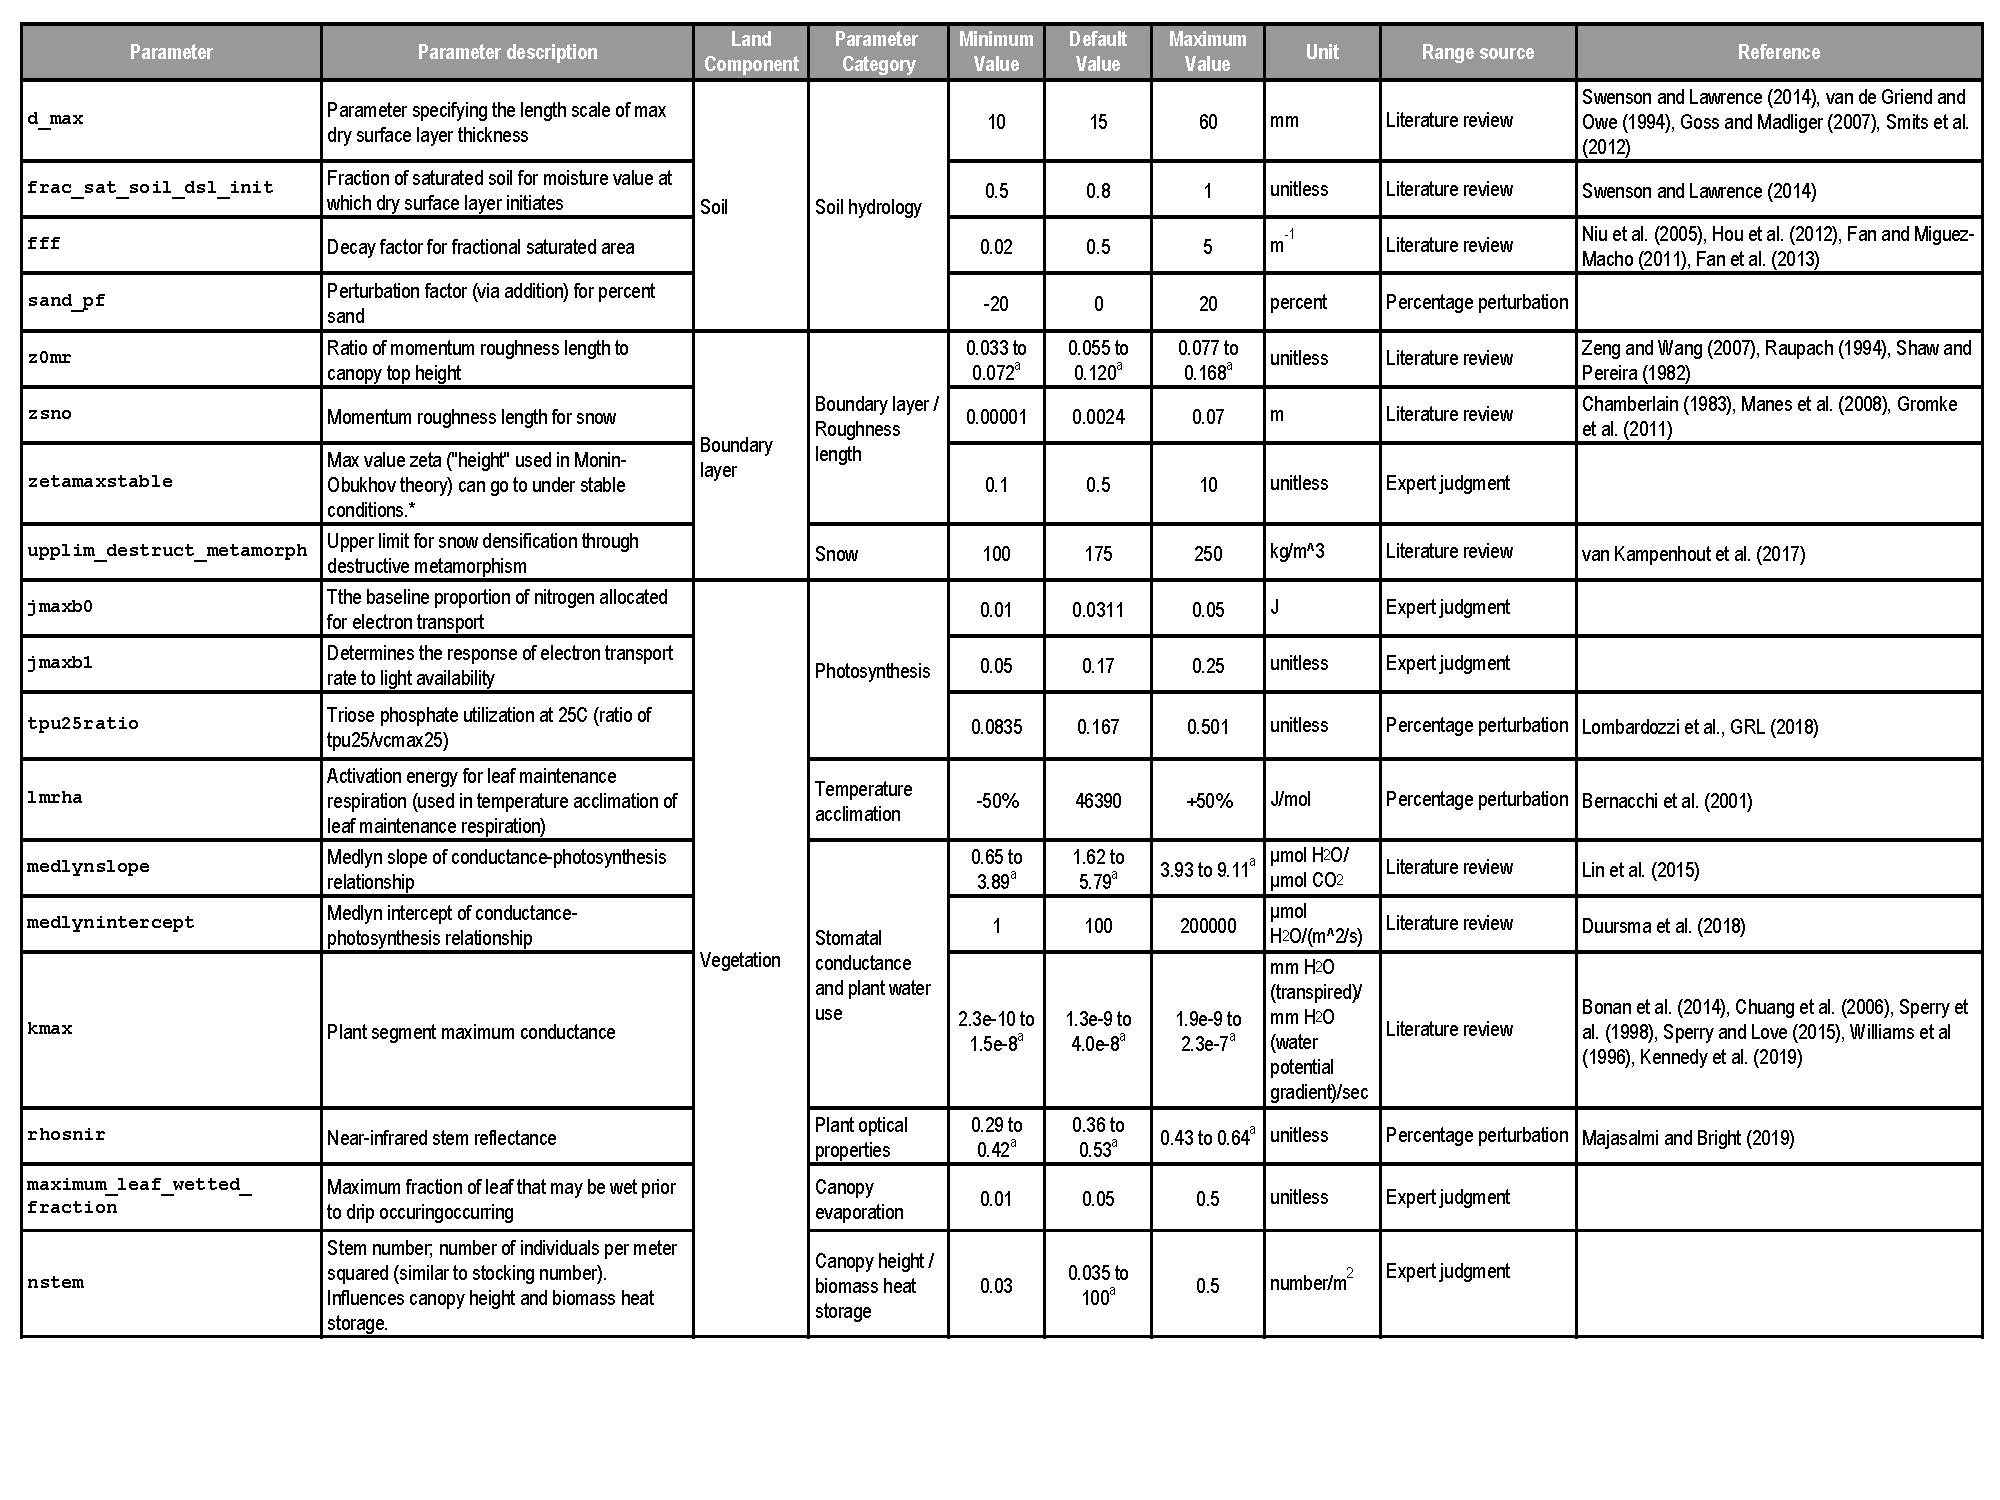
\includegraphics[width=\textwidth]{writing/figs/Table_Parameter_List.pdf}
  \caption{Land parameters used in this study. 
  $^a$Parameter ranges vary depending on the plant functional type.}
 \label{table:param_list}
 \end{sidewaystable}


%% ------------------------------------------------------------------------ 


%% ------------------------------------------------------------------------ 
%\bibliography{agusample}

\end{document}